\documentclass[main]{subfiles}

\newcommand{\degc}{$^\circ$C}

\begin{document}

\chapter{Barómetro}
\label{chap:barometro}

Como instrumento para determinar la altura del cuadricóptero se pensaba utilizar un GPS. La frecuencia de muestreo del GPS y el error en los datos provenientes del mismo lo hacen insuficiente como medio para estimar la elevación del cuadricóptero. Esta fue la motivación para la incorporación de un barómetro.

Las características principales del GPS son:
\begin{itemize}
\item Permite obtener un valor para la altura absoluta, libre de bias, pero hace falta promediar muestras durante varios minutos antes de llegar a un datos confiable.
\item  La precisión del GPS es mala muy cerca del suelo, lo cual representa un problema al intentar despegar y/o aterrizar.
\end{itemize}

Se opta por incorporar un barómetro, ya que aparentemente dichos sensores padecen de \textit{otros} problemas, y pueden complementar al GPS.

El sensor adquirido es un barómetro digital BOSCH BMP085. Permite medir presión absoluta, y, conociendo la presión y la temperatura a nivel del mar, permite calcular la altura absoluta.

Tiene varios modos de funcionamiento, habiendo un compromiso entre el consumo, la tasa de actualización, y la resolución.

\section{Objetivos}
%\ref{} agregar refs

El objetivo de estas pruebas es determinar como ha de usarse el barómetro BOSCH BMP085, incorporado para asistir en la determinación de la altura del cuadricóptero. Para ello se procede a caracterizar el sensor.

Se analizan las siguientes situaciones:

\begin{itemize}
\item Reposo: Se analizan períodos de distinta duración, para cumplir con distintos objetivos:
  \begin{itemize}
  \item Decenas de minutos: Caracterizar el drift y el tiempo de \textit{warm-up}.
  \item Decenas de segundos: Caracterización del ruido de las medidas.
  \end{itemize}
\item Altura relativa: 3 experimentos variando el rango a analizar: Puntos que distan decenas de centímetros entre sí, 1m entre sí, y aproximadamente 5m entre sí.
\end{itemize}

\newpage
\section{Materiales}
\label{sec:materiales}

\begin{itemize}
\item Laptop.
\item Tanza.
\item Cinta métrica.
\item Cubo de lapacho.
\item IMU ``Mongoose'' de CKDevices (cuenta con un BMP085).
\end{itemize}

\section{Consideraciones previas}
\label{consideraciones}

El sensor de presión devuelve la presión absoluta. Si se conoce la presión y la temperatura a nivel del mar, es posible calcular la elevación.

A nivel de la tropósfera, la capa más baja de la atmósfera, se puede calcular la altura a partir de la presión atmosférica mediante la siguiente fórmula\cite{bib:alt-press}:

\begin{equation}
  \label{eq:press-alt}
  p = p_0 \cdot \left(1 - \frac{L \cdot h}{T_0} \right)^\frac{g \cdot M}{R \cdot L}
\end{equation}

Donde:
\begin{itemize}
\item p0: 	Presión atmosférica estándar a nivel del mar -	101325 Pa.
\item L :	Gradiente de temperatura\footnote{Tasa de incremento de la temperatura con la altura (es negativa).} -	0.0065 K/m
\item T0:	Temperatura estándar a nivel del mar -	288.15 K
\item g :	Constante de gravitación universal -	9.80665 m/s2
\item M :	Masa molar del aire seco -	0.0289644 kg/mol
\item R :	Constante universal de los gases - 	8.31447 J/(mol$\cdot$K)
\end{itemize}


\section{Procedimiento}
\label{sec:procedimiento}

\subsection{Drift y \textit{warm-up}}
\label{sec:drift-y-warm-up}

En los datos tomados durante varios minutos, se observa lo que parecería ser un drift en las medidas obtenidas del barómetro. Se toman muestras durante 1 hora, con el barómetro quieto, comenzando con el circuito en frío\footnote{Habiendo estado apagado durante, por lo menos, los 30 minutos previos a la prueba.}.

\subsection{Caracterización del ruido}

Es de interés caracterizar el ruido en los datos provenientes del barómetro. Si se trata de un proceso estacionario, y de ruido blanco, entonces, promediando se puede reducir el error.

Se analizan datos tomados durante diversos períodos de tiempo: 5 minutos, 2 minutos, 20 segundos y 15 segundos.

Se analiza la autocorrelación de las muestras, y se compara el ruido con los valores dados por la hoja de datos. La hoja de datos especifica ruido RMS típico para los distintos modos de funcionamiento.

\subsection{Medidas de altura absoluta}

\begin{wrapfigure}{r}{0.25\textwidth}
\vspace{-70pt}
  \begin{center}
	\subfloat[Toma de datos.]{\label{fig:escalera_compu.jpg}
	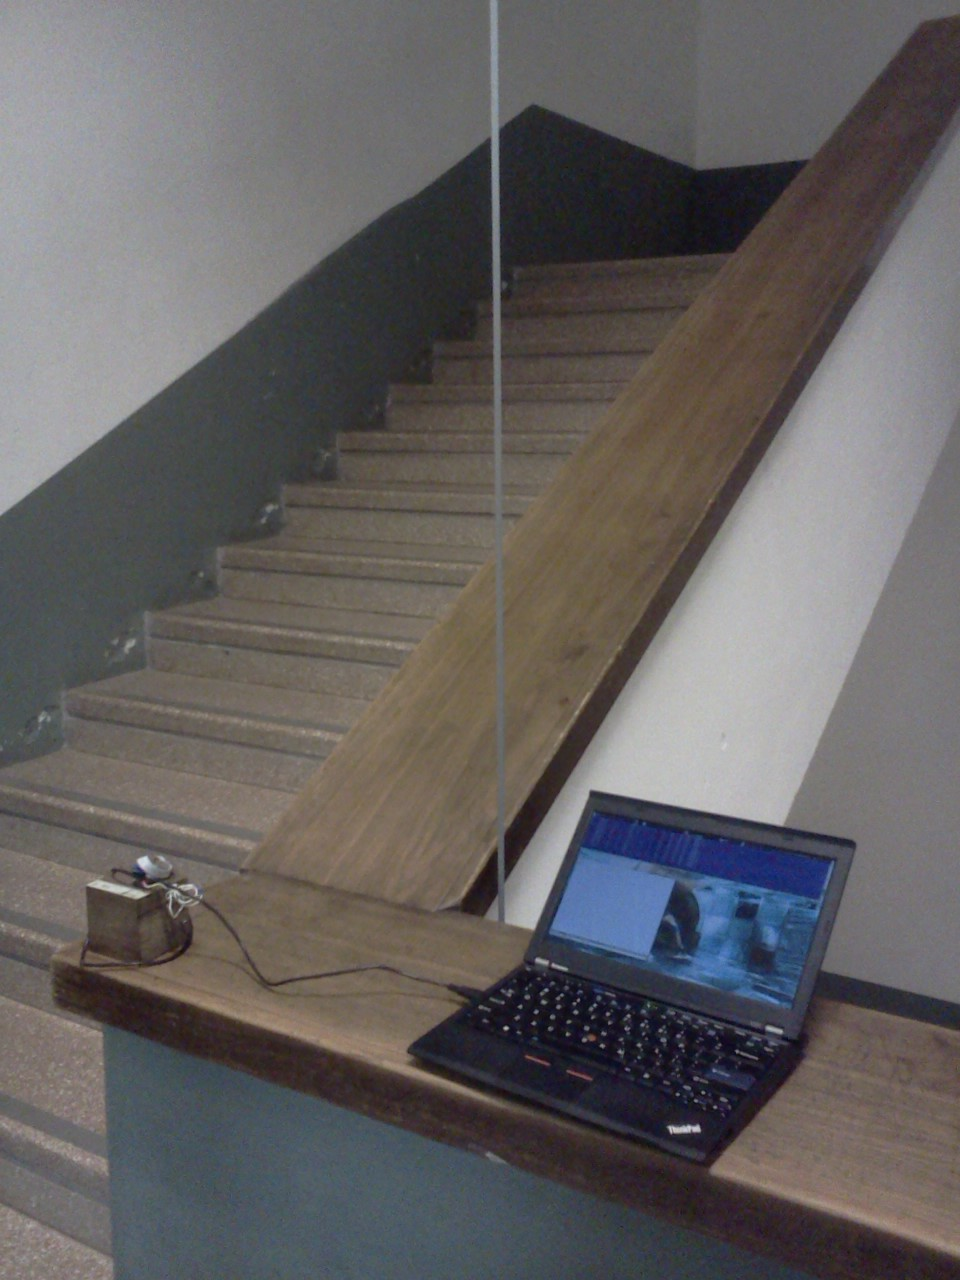
\includegraphics[width=0.2\textwidth]
		{./pics_barom/escalera_compu.jpg}}\\
	\subfloat[Vacío de la escalera.]{\label{fig:escalera_pater.jpg}
	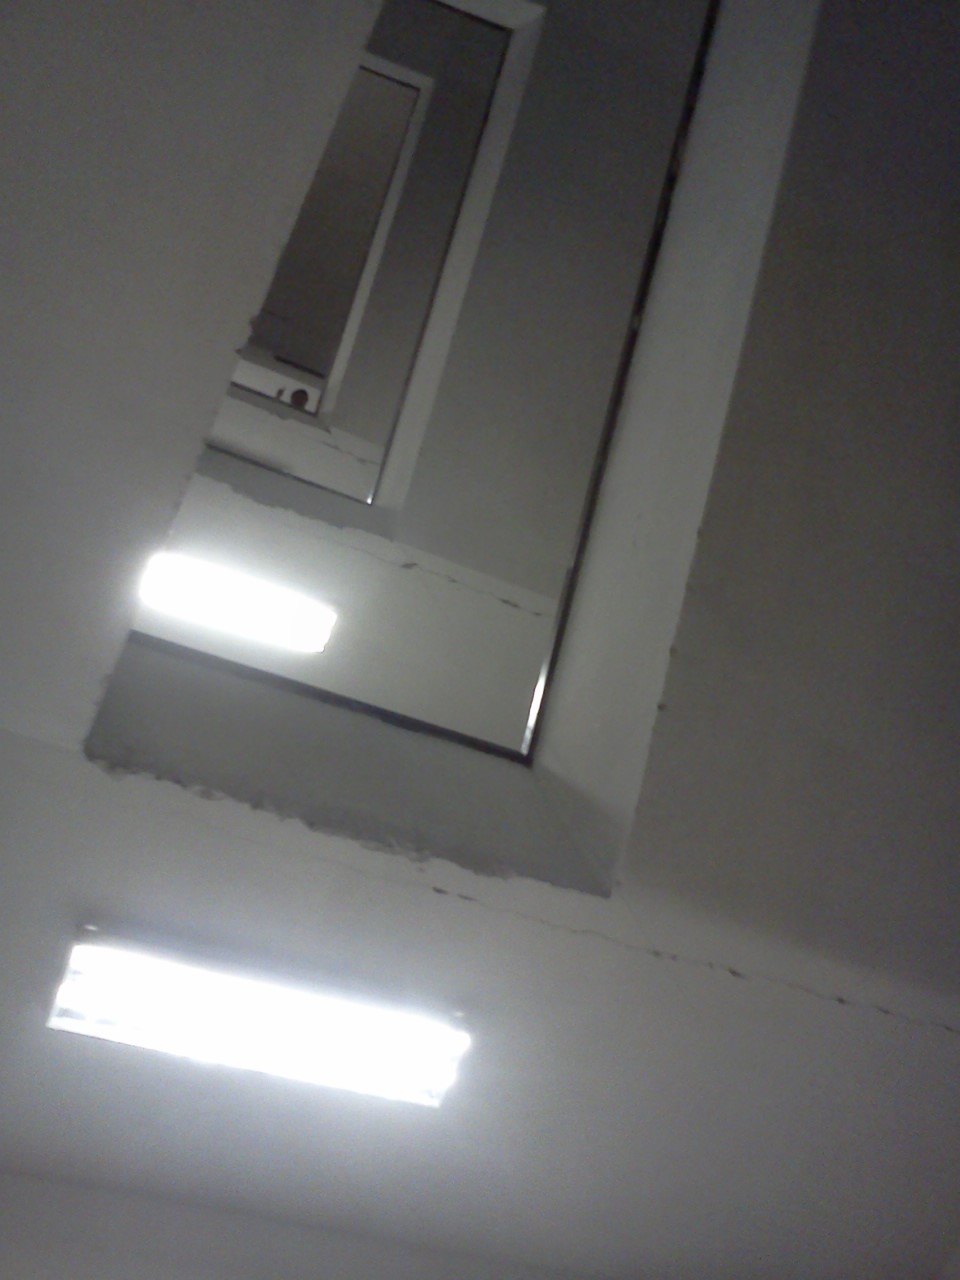
\includegraphics[width=0.2\textwidth]
		{./pics_barom/escalera_pater.jpg}}
  \end{center}
\vspace{-15pt}
  \caption{}
\label{fig:escalera-fing}
\vspace{-40pt}
\end{wrapfigure}

Para analizar la performance del barómetro como instrumento para determinar la elevación absoluta, se toman puntos de altura conocida, y se comparan las lecturas contra los datos conocidos.

\subsection{Distancias de varios metros}

Se deja despliega una cinta métrica en el vacío del centro de una escalera de 4 tramos en la Facultad de Ingeniería de la Universidad de la República. La cinta extendida cubre aproximadamente 25 metros. Se comparan las medidas dadas por el barómetro con las que se obtienen de la cinta.

Se utiliza una cinta de agrimensor, graduada cada 10 centímetros, para medir la distancia de un piso a otro. Luego se toman 1 minuto de datos en cada piso, recorriendo la escalera de un extremo a otro. Se repite este experimento 3 veces (se sube, se baja y se vuelve a subir) y luego se realiza un experimento similar, pero en lugar de detenerse a tomar muestras durante 1 minuto en cada piso, se apoya la IMU, se anota el tiempo (mediante software), y se sigue. La pausa en cada punto es menor a 2 segundos.

\subsection{Distancias de un metro}

\begin{wrapfigure}{r}{0.5\textwidth}
\vspace{-40pt}
\hspace{20pt}
  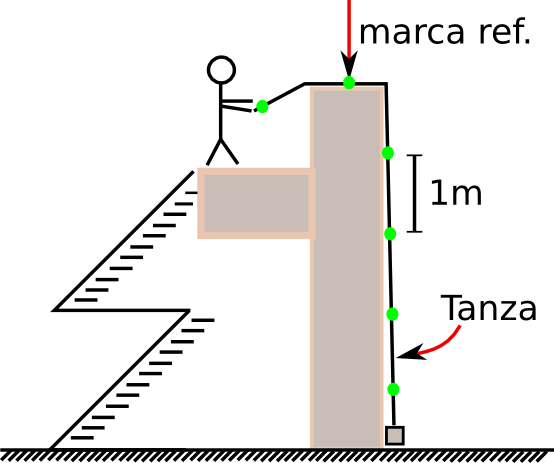
\includegraphics[width=.35\textwidth]{./pics_barom/imerl.png}
  \caption{Esquema experimento usando distancias de 1m.}
  \label{fig:imerl.png}
\vspace{-15pt}
\end{wrapfigure}

Se toma una tanza de pesca resistente. Se realizan marcas cada un metro, en seis puntos distintos de la tanza. En un extremo de la tanza se ata el cubo de lapacho, con la \emph{Mongoose} atornillada a él. Se lo deja descender desde la escalera del \emph{IMERL}\footnote{Instituto de Matemática y Estadística Rafael Laguardia}. Se suelta tanza hasta que el cubo se apoya contra el piso, de forma que la primer marca en la cuerda se encuentre junto a quien está realizando las medidas. Se hace una pequeña marca sobre la baranda, en el punto que coincide con la primer marca de la cuerda. Se mide la presión durante un minuto. Luego se sube el cubo hasta que la marca en la baranda coincida con la segunda marca de la cuerda (y por lo tanto el cubo subió 1 metro). Se vuelve a tomar la medida de presión. Se repite el procedimiento hasta tener la medida de presión a 5 alturas distintas. 
Se repite el experimento dos veces. Luego se toma la medida de presión a nivel del suelo. Se toman medidas mientras se sube y se baja el barómetro dos veces, se vuelven a tomar medidas a nivel del suelo.

\subsection{Distancias de decenas de centímetros}

Se ubica el cubo de lapacho siempre en la misma orientación sobre cada uno de los estantes de una estantería. Se coloca el cubo sobre el primer estante. Se mide la altura desde el suelo a la cara del cubo sobre la cual se encuentra apoyada la IMU. Se mide la presión durante 8 minutos. Se mueve el cubo al estante siguiente. Se vuelve a medir la altura respecto del suelo con un metro y se mide la presión durante un minuto. Se repite el procedimiento para cada uno los cinco estantes que componen la estantería. Luego se repite el experimento, pero tomando solamente 5 segundos de datos por estante.

\section{Análisis y resultados}

\subsection{Drift y \textit{warm-up}}
\label{sec:drift-y-warm-up}

Para observar si hay un drift y/o tiempo de \textit{warm-up} significativo, se procede a tomar muestras durante 1 hora, habiendo estado el dispositivo desenchufado durante por lo menos media hora (el circuito arranca en frío).

Se repite este experimento varias veces. En las figuras \ref{fig:1hora_04.pdf} y \ref{fig:1hora_01.pdf} se observan los resultados característicos.

\begin{figure}[h!]
\hspace{-50pt}
\subfloat[Muestras durante una hora, experimento \#1.]{\label{fig:1hora_01.pdf}
  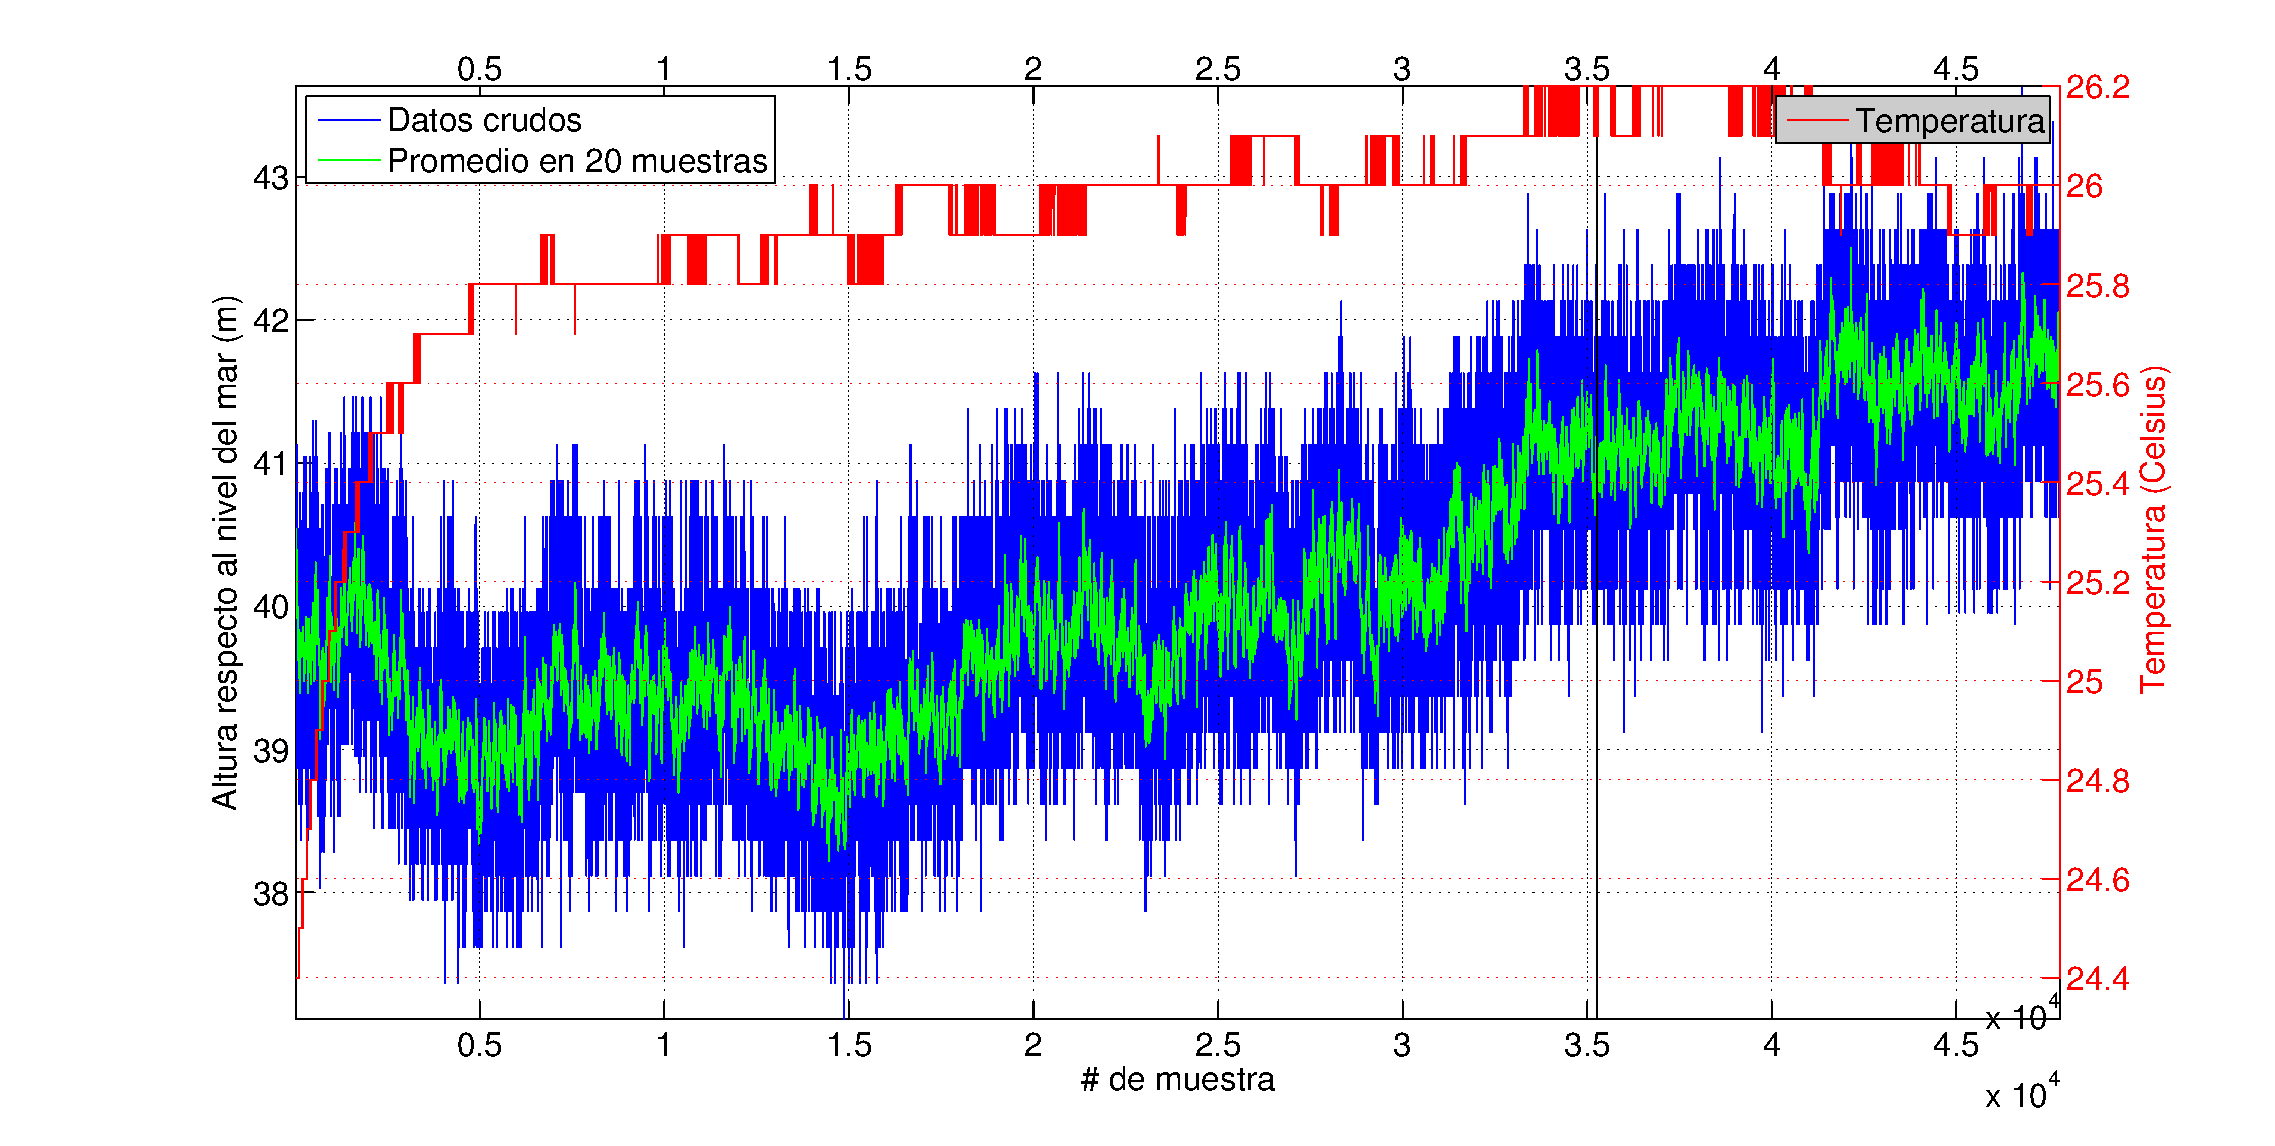
\includegraphics[width=.6\textwidth]{./pics_barom/1hora_01.pdf}}
\subfloat[Muestras durante una hora, experimento \#4.]{\label{fig:1hora_04.pdf}
  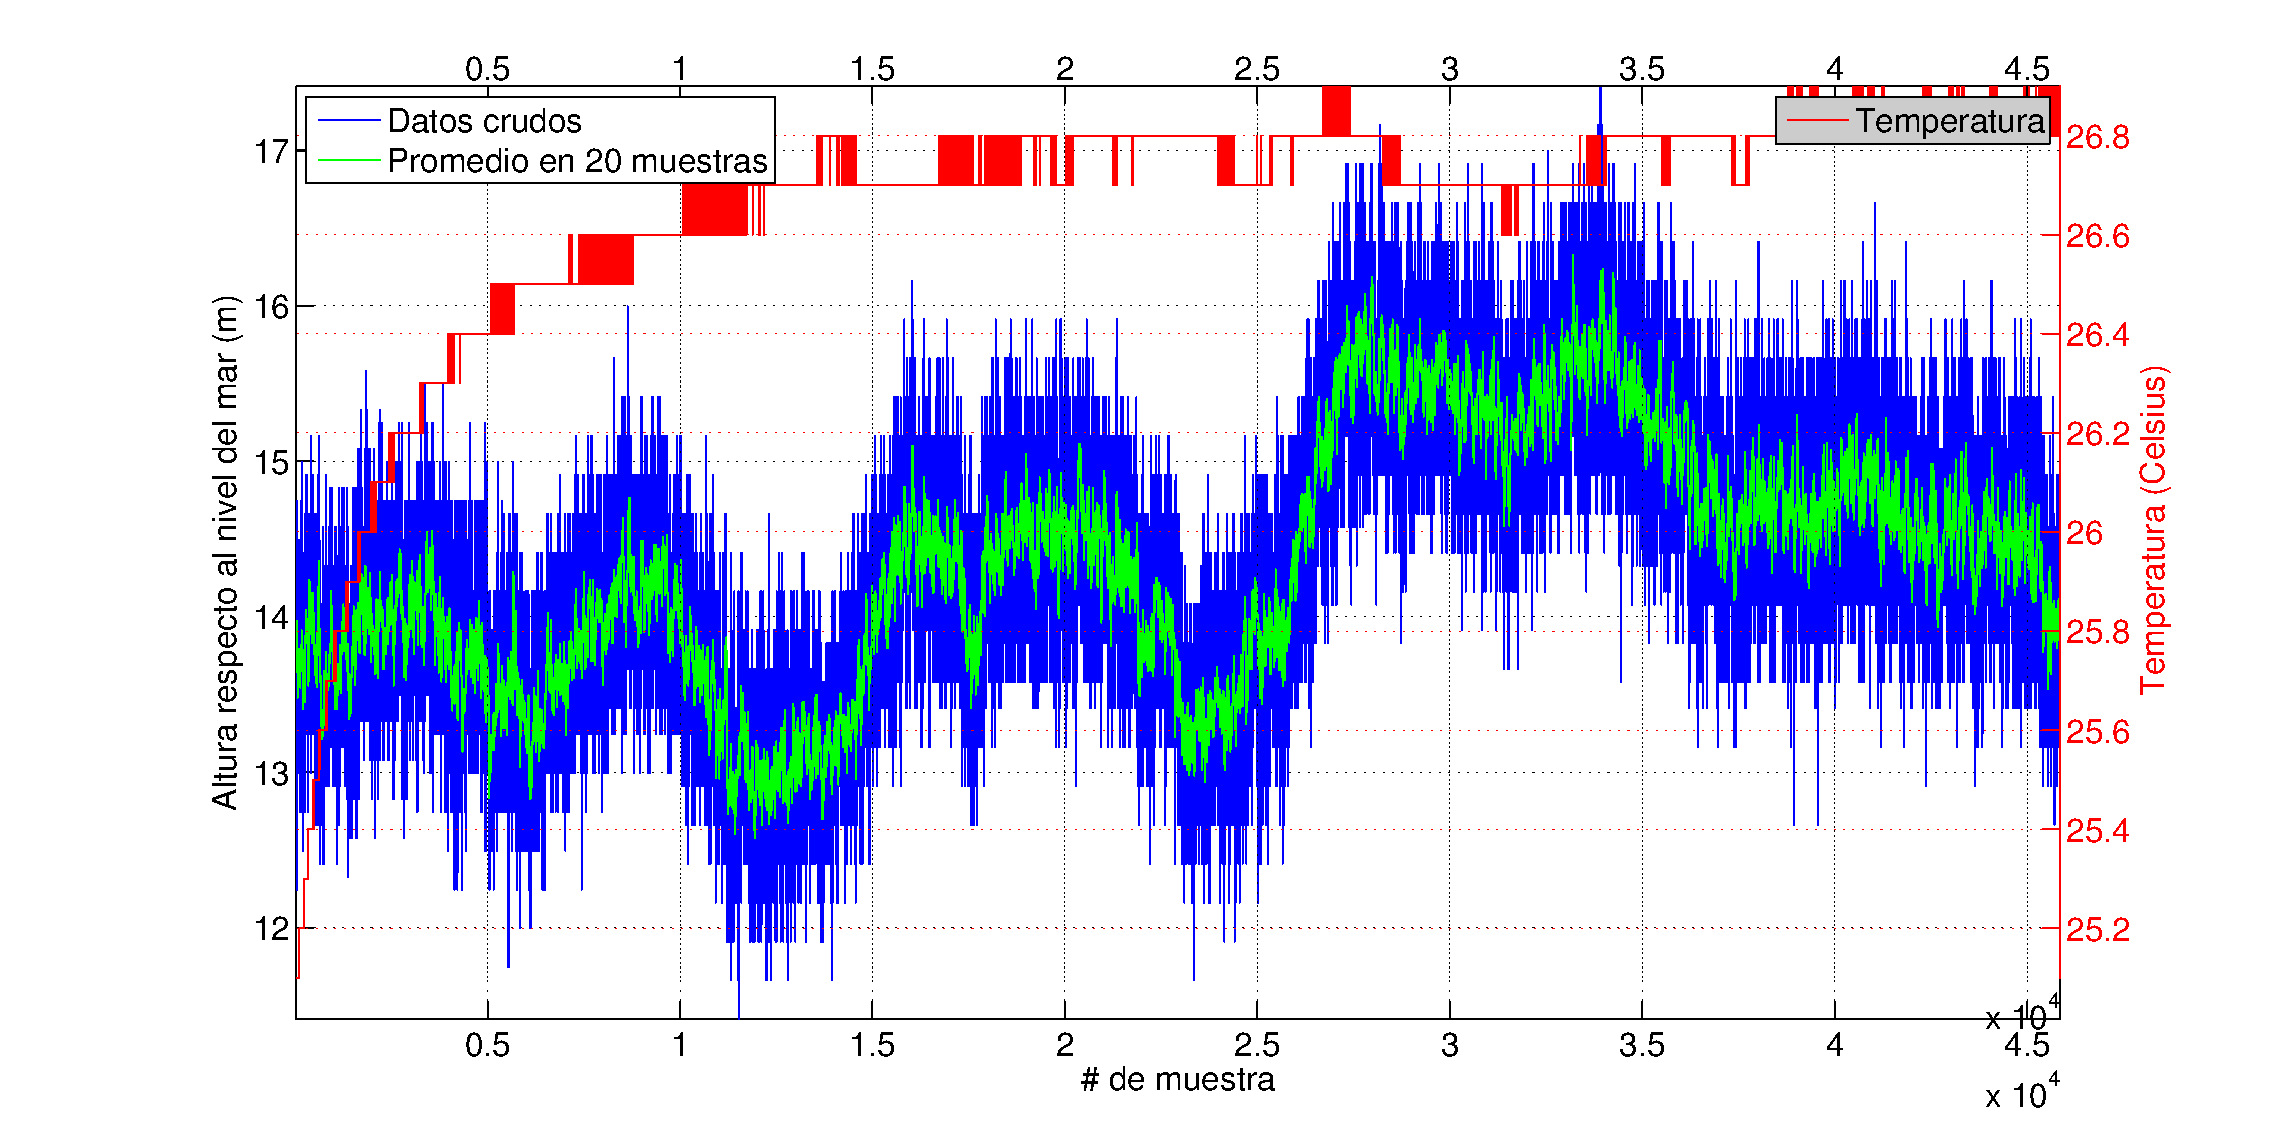
\includegraphics[width=.6\textwidth]{./pics_barom/1hora_04.pdf}}
\caption{}
\end{figure}
\vspace{-10pt}

Se observa que existe un tiempo de \textit{warm-up} bastante extenso, pero con un rango pequeño. La temperatura tarda entre 15 y 45 minutos en estabilizarse, y en el proceso varía menos de 2\degc. Las muestras del barómetro no parecen estar directamente correlacionadas con la temperatura.

El barómetro no parece ser adecuado para medir la elevación absoluta. En los datos de las figuras \ref{fig:1hora_01.pdf} y \ref{fig:1hora_04.pdf} se observan variaciones de hasta 3 metros en la estimación de la altura en un período de 1 hora. Sin embargo, el error en el corto plazo es significativamente menor que en el largo plazo, parece viable el uso del barómetro como estimador de la altura en el corto plazo. Esto se analiza más adelante.

\subsection{Caracterización del ruido}
\label{sec:caract-ruido}

En los logs de la sección \ref{sec:drift-y-warm-up}, se observa que:
\begin{itemize}
\item El comportamiento del ruido en intervalos extensos no es estacionario.
\item La mayoría de los saltos en la medida de la altura son de aproximadamente 25cm. Esto no es coherente con las especificaciones dan una resolución de 1Pa, que corresponden a una variación en altura de aproximadamente 8cm.
\end{itemize}

\subsubsection{Estacionareidad}

Analizando el ruido en intervalos más pequeños, donde el proceso se puede considerar estacionario, el comportamiento del ruido es muy similar al del ruido blanco.

En la figura \ref{fig:autocorr} se observa la autocorrelación de la muestras tomadas del barómetro en intervalos de tiempo de 5 minutos, 2 minutos, y 15 segundos.

Cabe destacar que el ruido se puede considerar estacionario si se usan intervalos de tiempo menores a 15 segundos.

\begin{figure}[H]
\vspace{-20pt}
\centering
	\subfloat[5 minutos]{\label{fig:autocorr_5m.pdf}
	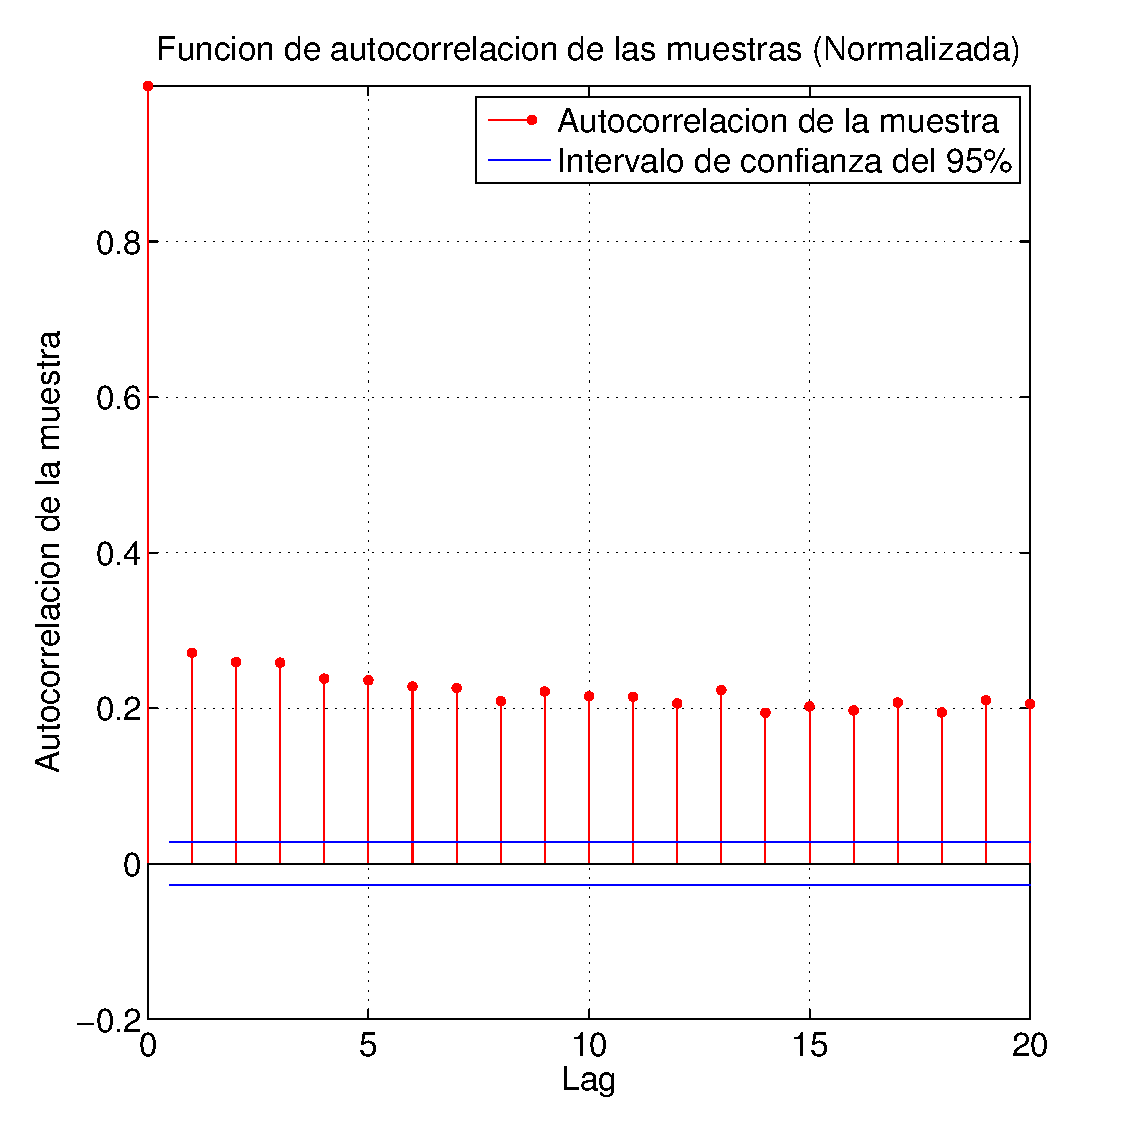
\includegraphics[width=0.3\textwidth]
		{./pics_barom/autocorr_5m_log04.pdf}}
	\subfloat[15 segundos]{\label{autocorr_15s_log04.pdf}
	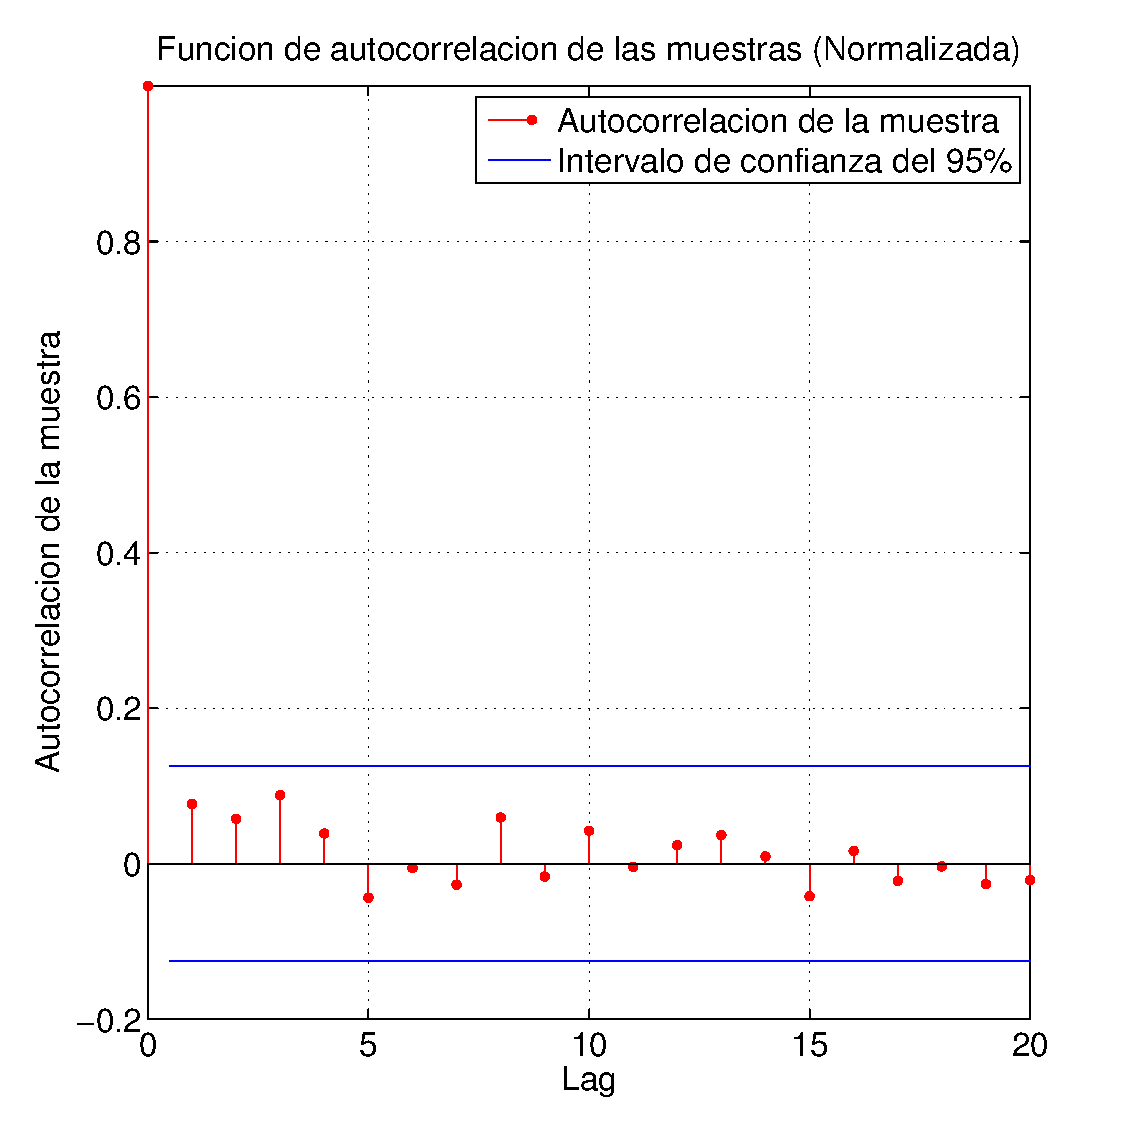
\includegraphics[width=0.3\textwidth]
		{./pics_barom/autocorr_15s_log04.pdf}}
	\subfloat[15 segundos]{\label{autocorr_15s_log04.pdf}
	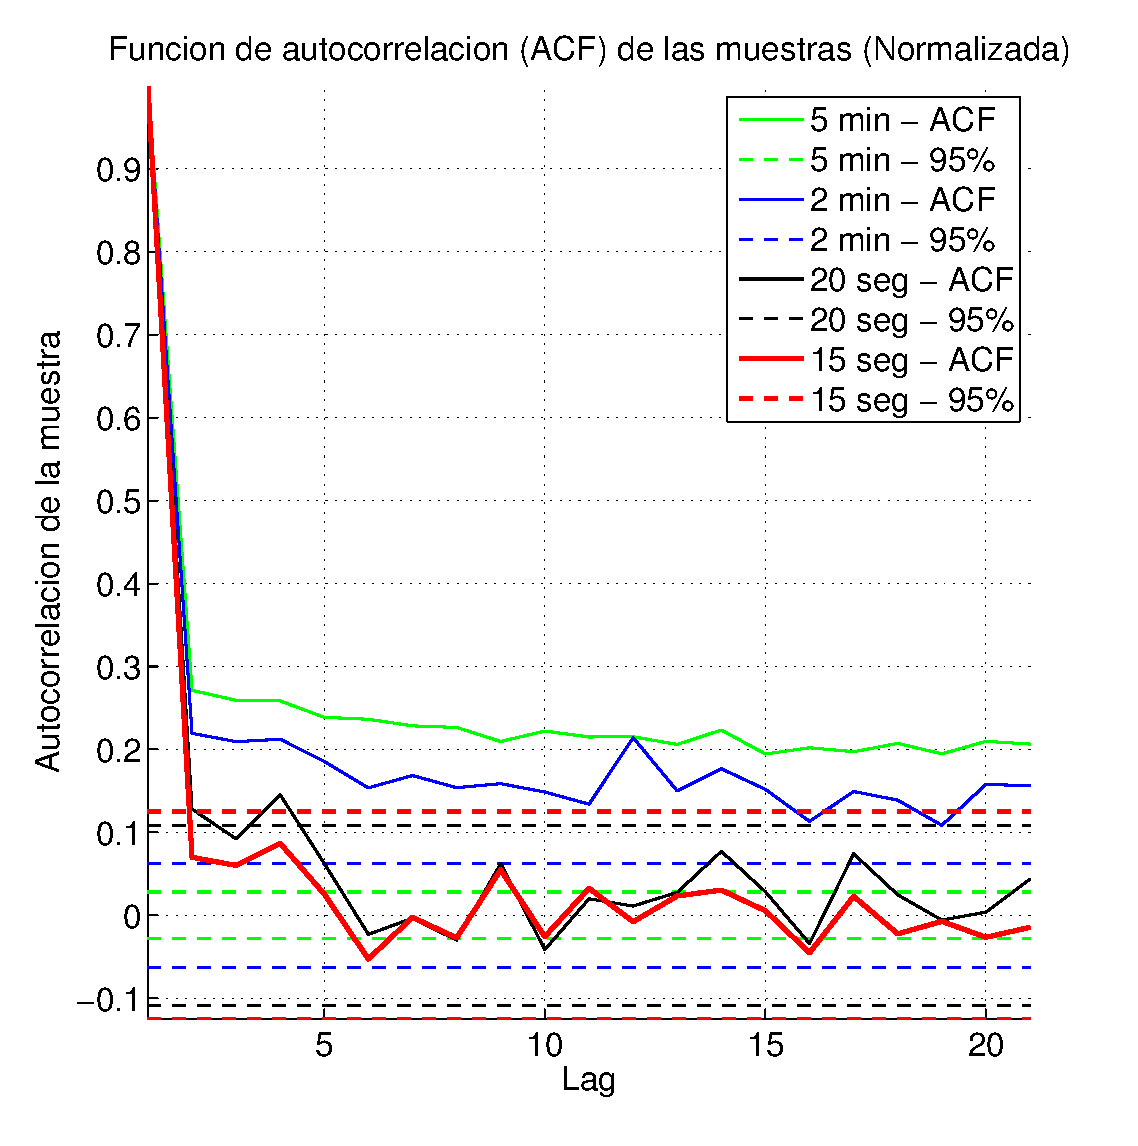
\includegraphics[width=.3\textwidth]
		{./pics_barom/autocorr.pdf}}
  \caption{Autocorrelación de las muestras del barómetro.}
\label{fig:autocorr}
\end{figure}
\vspace{-20pt}

\subsubsection{Modos de funcionamiento}

\begin{wraptable}{r}{0.6\textwidth}
\vspace{-40pt}
\centering
\begin{tabular}{c|c|c|c|} 
\cline{2-4}
	& \multicolumn{3}{|c|}{\cellcolor[gray]{0.8} Ruido RMS  (m)}      \\ \hline
\multicolumn{1}{|c|}{\cellcolor[gray]{0.8} {Modo}} & \cellcolor[gray]{0.8} {$\mu p$} &\cellcolor[gray]{0.8} {Sensor} &\cellcolor[gray]{0.8} {specs}\\ \hline

\multicolumn{1}{|c|}{0}	&	0.52	&	0.52	&	0.50\\
\hline
\multicolumn{1}{|c|}{1}	&	0.37	&	0.45	&	0.40\\
\hline
\multicolumn{1}{|c|}{2}	&	0.25	&	0.37	&	0.30\\
\hline
\multicolumn{1}{|c|}{3}	&	0.63	&	0.35	&	0.25\\
\hline

\end{tabular}
\caption{}
\vspace{-15pt}
\label{tab:ruido-rms}
\end{wraptable}

El barómetro permite trabajar en varios modos. Básicamente, permite que se le exija más resolución, menos ruido, y a cambio aumenta el tiempo que tarda en tener un dato nuevo listo, y consume más energía. Esto lo logra promediando datos internamente. En la tabla \ref{tab:ruido-rms} se compara el ruido RMS en los distintos modos, con lo que se lograría usándolo en el modo básico (sin promediar internamente) y promediando en el microprocesador.

La resolución más atractiva parece ser la número 2, en la cual se promedian 4 datos. Se concluye que, si se dispone de procesador se optará por promediar datos en él, de lo contrario se usará el promedio calculado por el sensor.

\newpage
\subsubsection{Resolución del instrumento}

En la figura \ref{fig:barom_hist_exp4.pdf} se observa un histograma de las diferencias entre muestras sucesivas de los datos del barómetro. Se observa que la mayor parte de los datos saltan de a 25cm. Se esperaba una discretización en niveles de  aproximadamente 8cm, correspondientes a variaciones de presión de 1Pa (la resolución del instrumento).

Puede resultar difícil ver que hay muestras en todos los bins, pero mirando con detalle se puede. Puede deberse a un problema de software, o la construcción del sensor en sí. Este problema no parece ser significativo.

\subsection{Altura absoluta}

Las figuras \ref{fig:1hora_01.pdf} y \ref{fig:1hora_04.pdf} se corresponden a datos tomados a la misma altura, pero en dias distintos. Cabe destacar que la diferencia entre ambas curvas llega es de aproximadamente 25 metros.

Se descarta la posibilidad de utilizar el barómetro para determinar la altura absoluta, ya que estando el barómetro a una altura fija, la elevación varía mucho de un día a otro, lo cual refleja una fuerte dependencia con factores externos, probablemente climáticos, que no interesa considerar.

\subsection{Distancias de varios metros}

En las siguientes figuras se observan los resultados del experimento. Las líneas verticales (en negro) representan el comienzo y el fin de la toma de datos en cada piso. No se hace una medida de la altura absoluta, se miden las distancias entre piso y piso (con la cinta métrica), y se usa como origen de coordenadas la altura dada por el promedio de algunas muestras al comienzo del experimento, ya sea en el piso de más arriba, o en el piso de más abajo (bajadas y subidas respectivamente). La coordenada Y de los segmentos en rojo que unen las rectas verticales representan la distancia entre el origen y el piso actual. Dicha distancia se mide con la cinta métrica.

\begin{figure}[h!]
\centering
\subfloat[Subida \#1.]{\label{fig:metros-s1.pdf}
  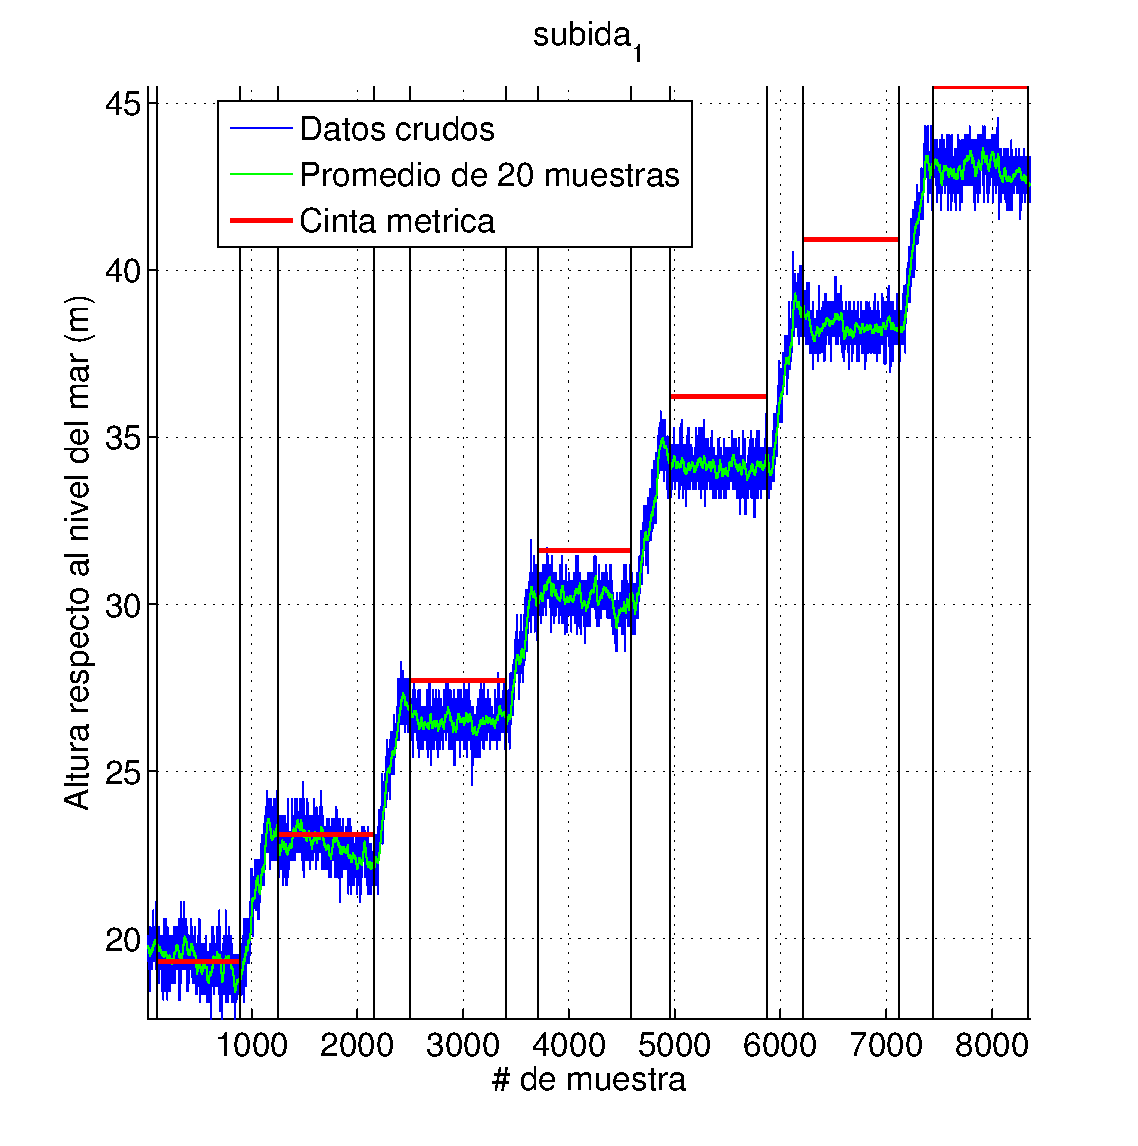
\includegraphics[width=.5\textwidth]{./pics_barom/metros-s1.pdf}}
\subfloat[Bajada \#1.]{\label{fig:metros-b1.pdf}
  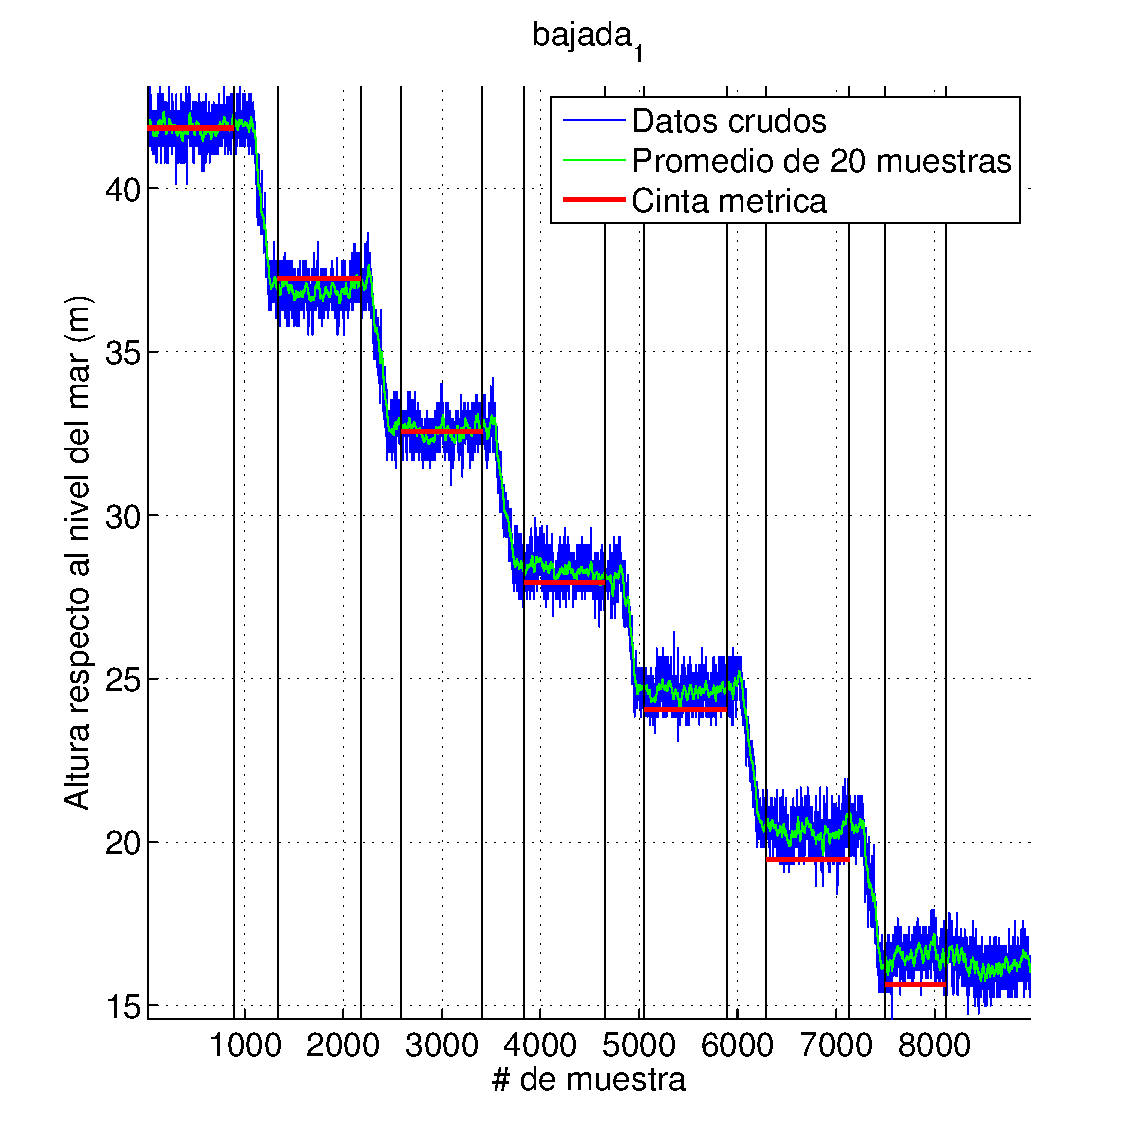
\includegraphics[width=.5\textwidth]{./pics_barom/metros-b1.pdf}}
\caption{Subida/Bajada \#1}
\end{figure}

En la figura \ref{fig:metros-s1.pdf} se observa que para cuando se termina de recorrer la escalera, el error acumulado se llega a los 3 metros. En la \ref{fig:metros-b1.pdf} se observan resultados mejores que en la figura \ref{fig:metros-s1.pdf}. Se repite la subida, y se obtienen resultados similares a los de la figura \ref{fig:metros-b1.pdf}, por este motivo no se incluye una figura de este último experimento.

Los errores en las medidas se analizan más adelante.

Cabe destacar que la performance en la figura \ref{fig:metros-rapido.pdf} es muy similar a la que se obtuvo tomando muestras durante 1 minutos. Esto resulta alentador, ya que se pretende utilizar el barómetro para obtener medidas con una frecuencia mucho mayor 1Hz.

En la figura \ref{fig:metros-err-accum.pdf} se observa la evolución del error acumulado para 2 subidas\footnote{No se incluye una gráfica de la segundo subida, ya es muy similar, en cuanto al error, a la de la primera bajada, pero con un error del orden del de la primer bajada.}, 1 bajada y una bajada rápida.

El error en la determinación de la distancia entre un piso y el siguiente se observa en la figura \ref{fig:metros-err-piso-a-piso.pdf}.

El error de la figura \ref{fig:metros-err-piso-a-piso.pdf} es relativo a la altura de cada piso, que son de aproximadamente 4.3m. Analizando los número con cuidado, se llega a que el error es siempre menor al 10\%.

De las figuras \ref{fig:metros-rapido.pdf} y \ref{fig:metros-err-accum.pdf} se desprende que utilizando promedios de 20 muestras\footnote{Esta es la cantidad de muestras que se promediaron para determinar la altura cada vez en cada piso en el experimento ``rápido''.}, se obtiene un error de aproximadamente 0.5m. El comportamiento del barómetro es aceptable, y se corresponde con las especificaciones de la hoja de datos.


\vspace{-10pt}
\begin{figure}[h!]
\centering
\subfloat[Bajada sin detenerse en cada piso.]{\label{fig:metros-rapido.pdf}
  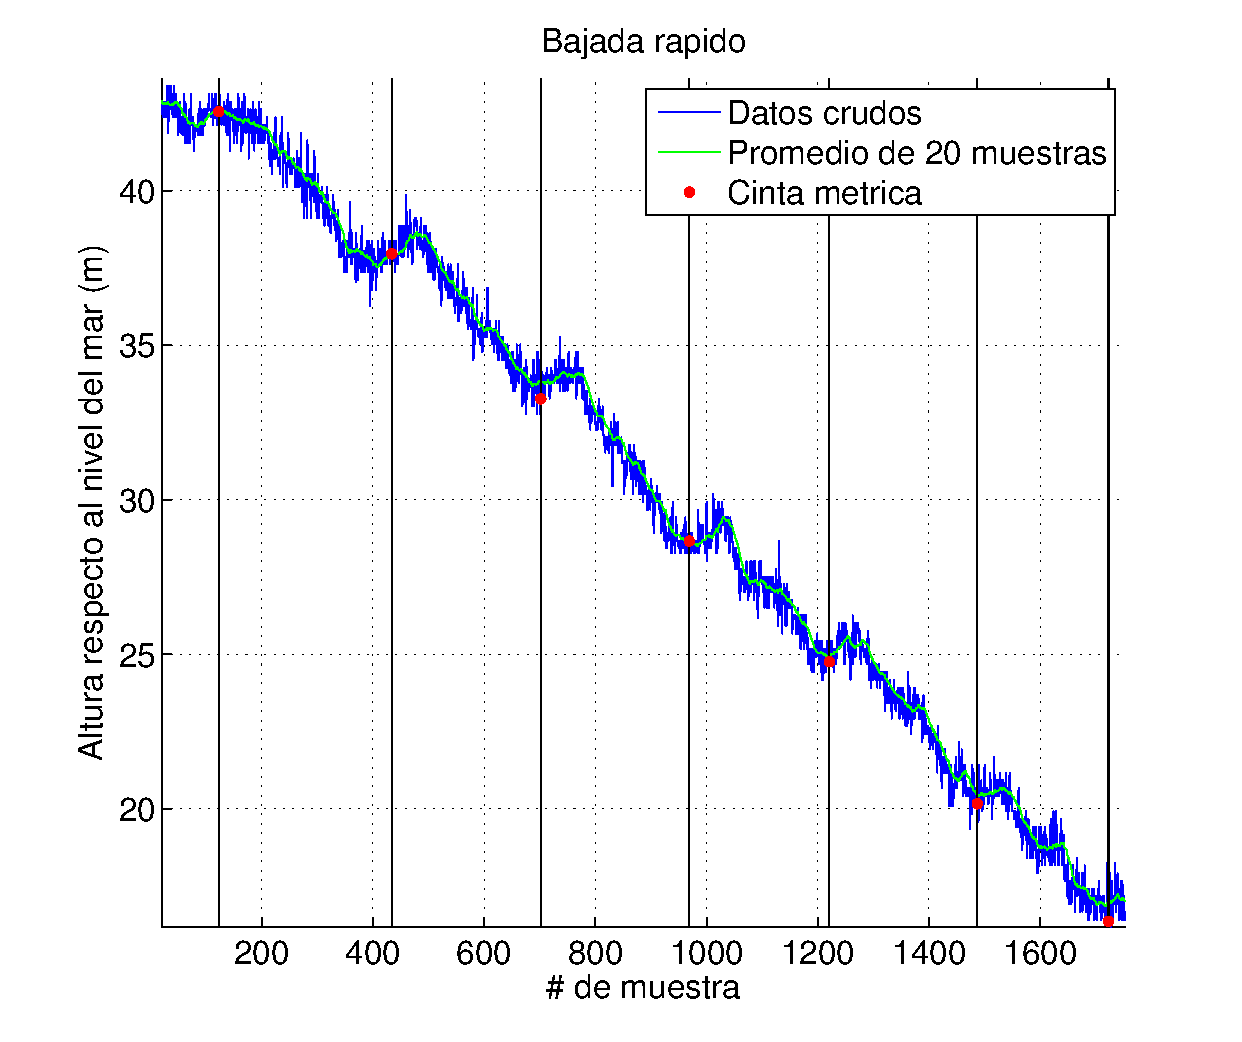
\includegraphics[width=.55\textwidth]{./pics_barom/metros-rapido.pdf}}
\subfloat[Histograma de las diferencias, experimento \#4.]{\label{fig:barom_hist_exp4.pdf}
  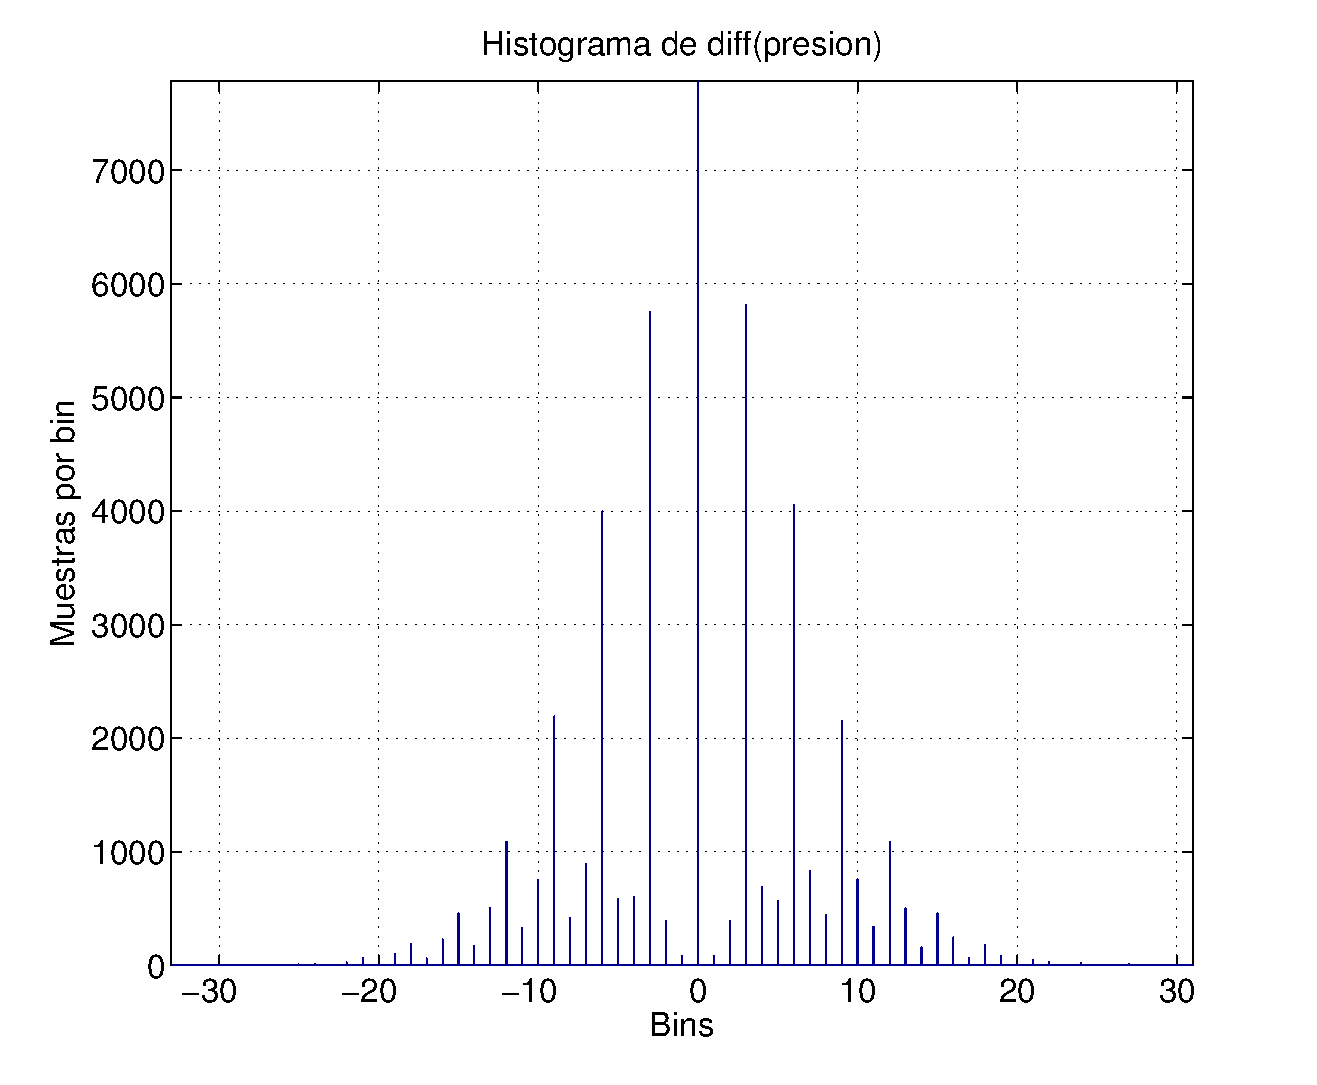
\includegraphics[width=.5\textwidth]{./pics_barom/barom_hist_exp4.pdf}}
  \caption{}
\end{figure}

\subsection{Distancias de un metro}

Las figuras \ref{fig:esc1.pdf} y \ref{fig:esc2.pdf} presentan las medidas obtenidas al realizar las medidas estáticas a alturas que difieren de un metro. La figura \ref{fig:variando} muestra las medidas obtenidas durante el proceso de subir y bajar el barómetro. En las tres figuras se observan los datos obtenidos y la media móvil considerando 20 muestras.

\begin{wrapfigure}{l}{0.75\textwidth}
\hspace{-40pt}
	\subfloat[Error acumulado.]{\label{fig:metros-err-accum.pdf}
	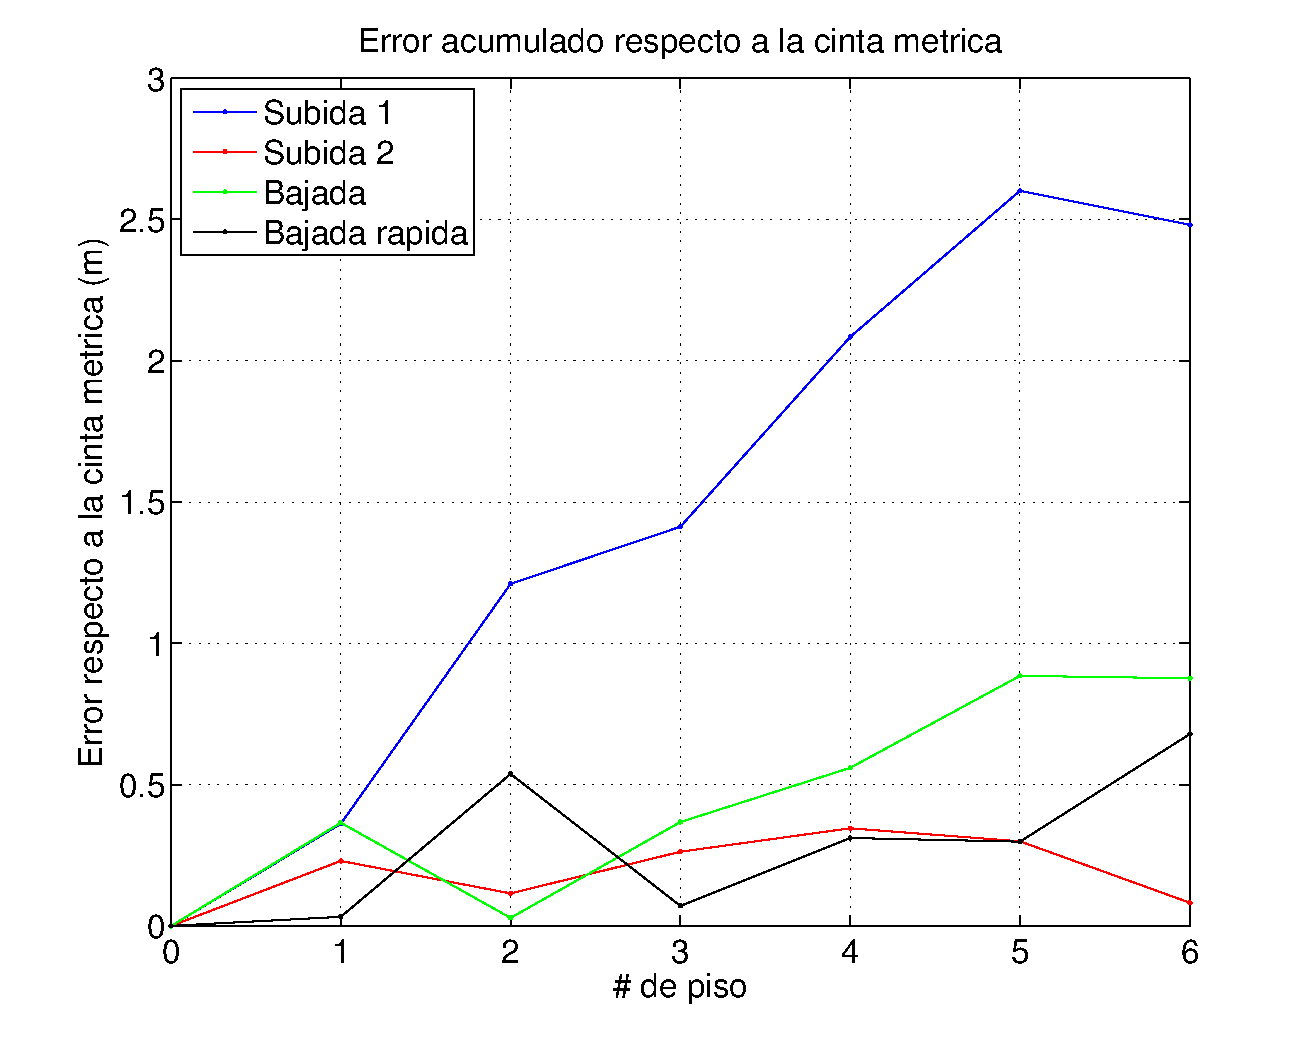
\includegraphics[width=.38\textwidth]
        {./pics_barom/metros-err-accum.pdf}}
	\subfloat[Error en la estimación de la distancia del piso anterior al actual.]{\label{fig:metros-err-piso-a-piso.pdf}
	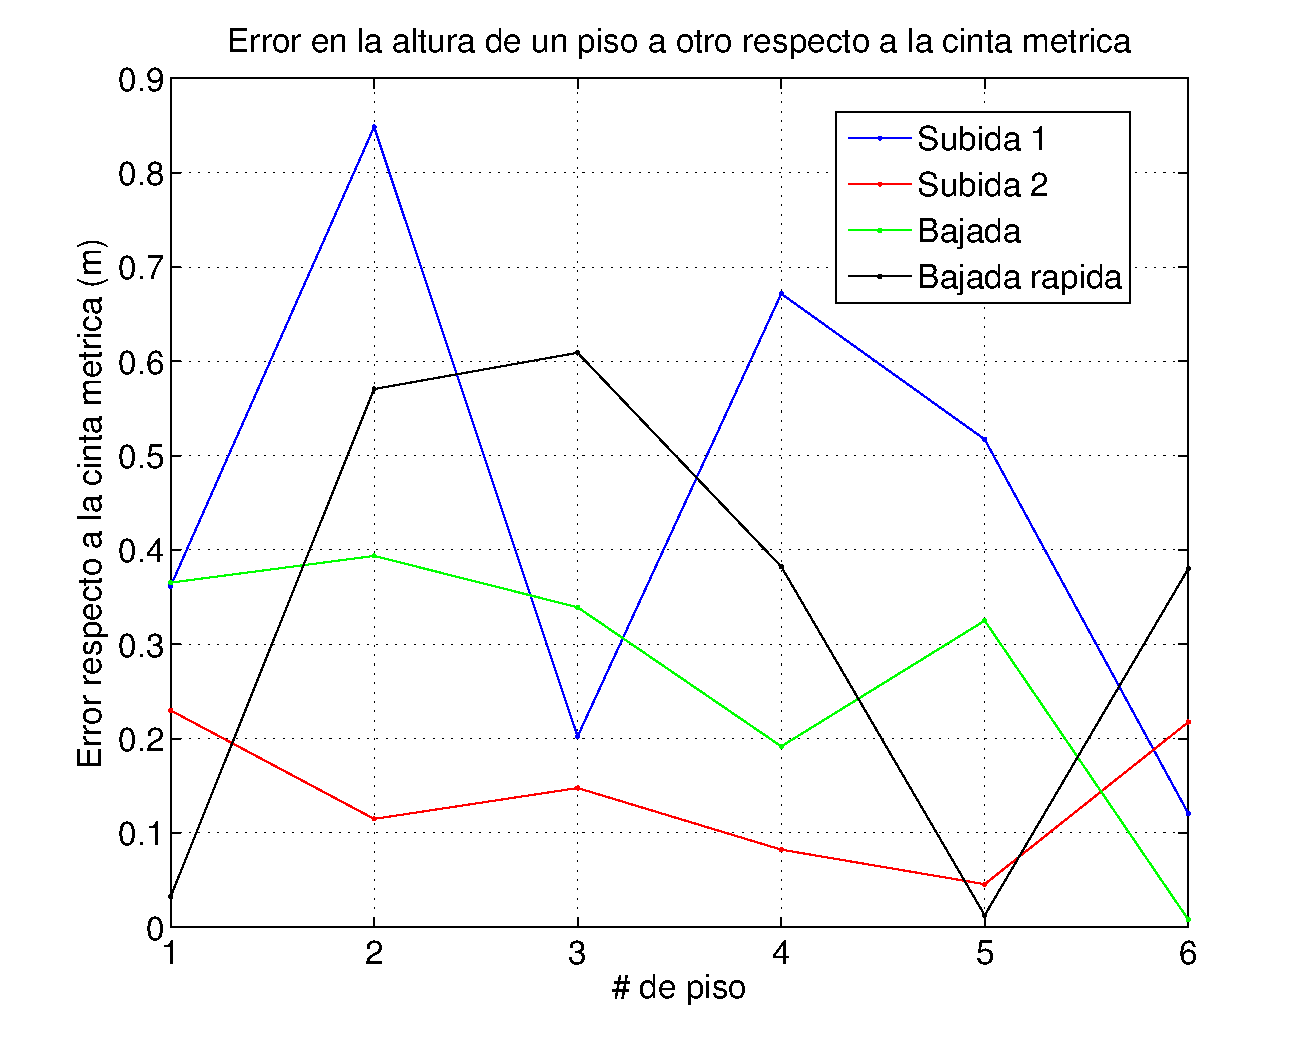
\includegraphics[width=.38\textwidth]
        {./pics_barom/metros-err-piso-a-piso.pdf}}
  \caption{Evolución del error en distancias de varios metros.}
\label{fig:autocorr}
\vspace{-15pt}
\end{wrapfigure}

Se aprecia que el comportamiento es acorde a lo esperado, corresponde a las acciones realizadas. Se analizan con mayor detenimiento los resultados para concluir que es lo que se puede esperar del barómetro.

En la tabla \ref{tab:alturasm} se muestran los valores de altura obtenidos en las distintas posiciones en las dos series de datos tomadas. La altura absoluta no tiene sentido, ya que no se conoce la presión a nivel del mar en el momento de tomar las muestras, por lo tanto la ecuación \ref{eq:press-alt} no dará el resultado correcto.

\begin{figure}[H]
\vspace{-14pt}
\hspace{-30pt}
	\subfloat[Primer serie de medidas cada 1 metro.]{\label{fig:esc1.pdf}
  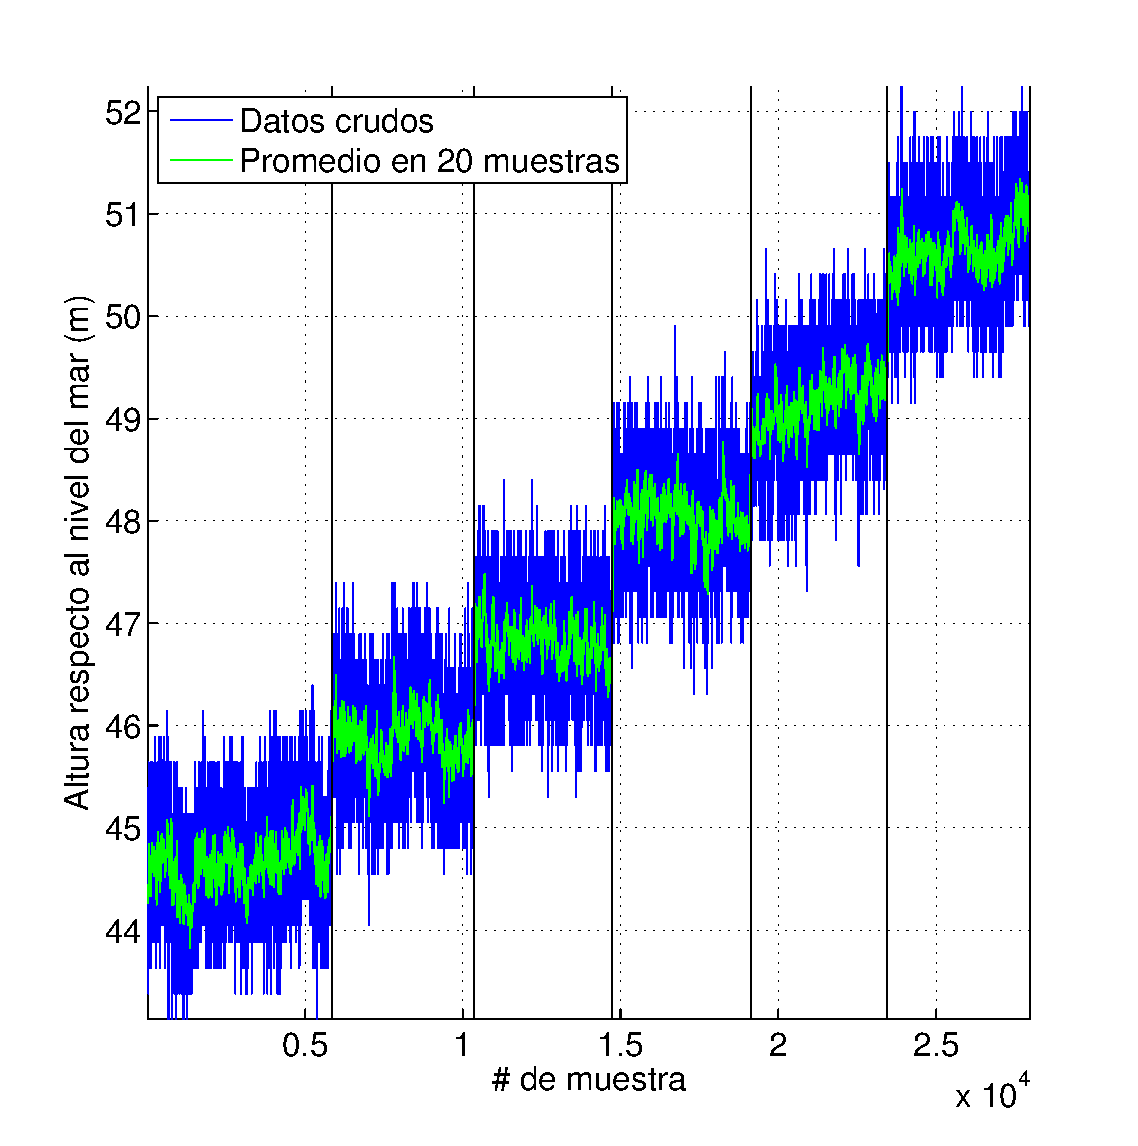
\includegraphics[width=.5\textwidth]{./pics_barom/esc1.pdf}}
	\subfloat[Segunda serie de medidas cada 1 metro.]{\label{fig:esc2.pdf}
  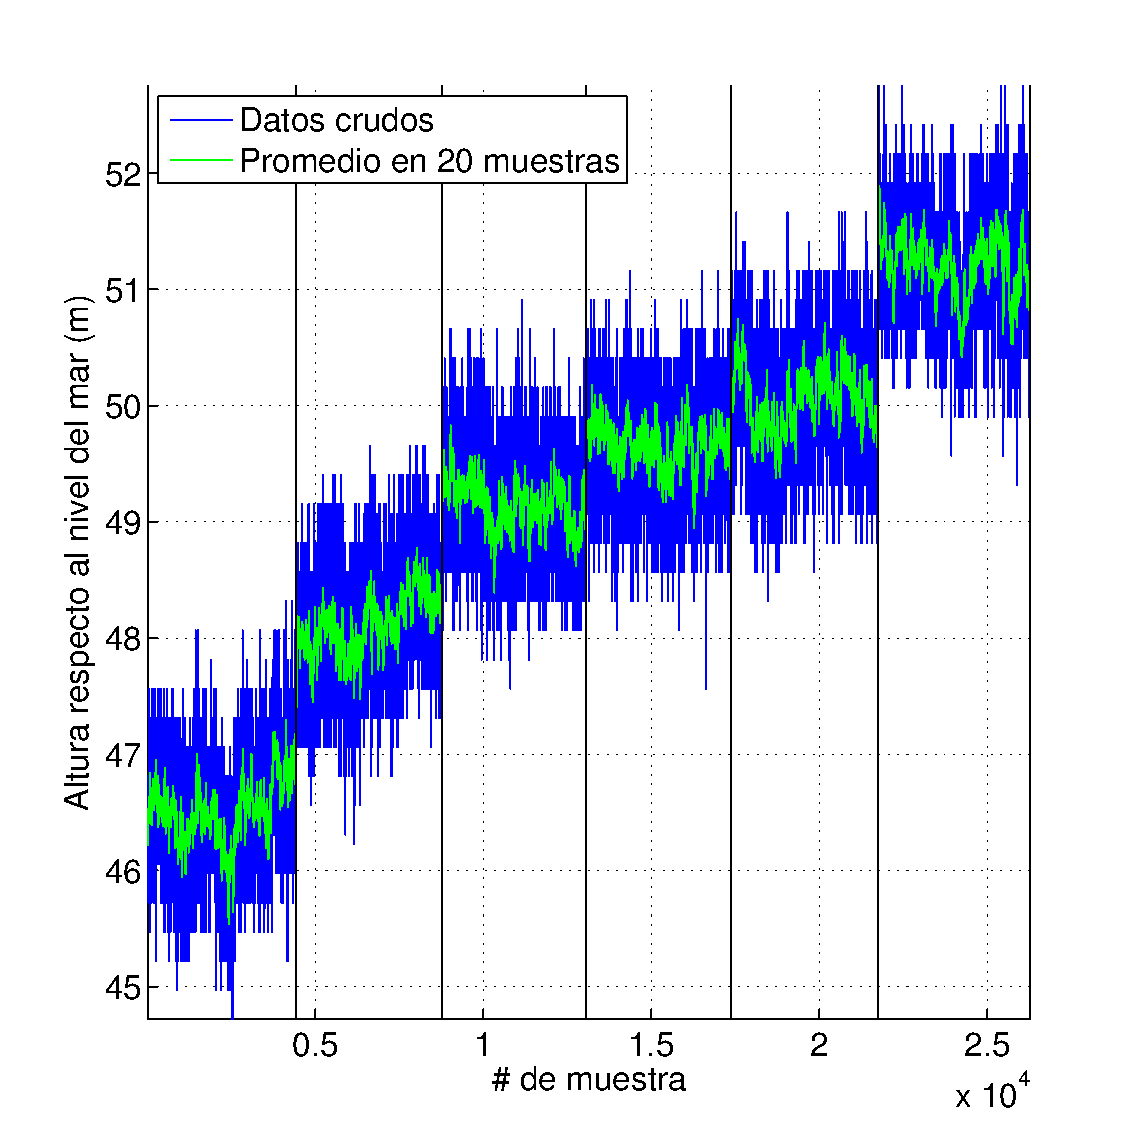
\includegraphics[width=.5\textwidth]{./pics_barom/esc2.pdf}}
  \caption{Experimento: Distancias de 1 metro.}
\label{fig:1m}
\end{figure}

\vspace{-10pt}
\begin{wraptable}{l}{0.45\textwidth}
\begin{tabular}{c|c|c|} 
	& \multicolumn{2}{|p{100pt}|}{\cellcolor[gray]{0.8} Altura medida con el barómetro (m)}      \\ \hline
\cellcolor[gray]{0.8} {Posición} & \cellcolor[gray]{0.8} {Serie 1} &\cellcolor[gray]{0.8} {Serie 2}\\ \hline

\multicolumn{1}{|c|}{1} & 44.66 & 46.52 \\ \hline
\multicolumn{1}{|c|}{2} & 45.87 & 48.12\\ \hline
\multicolumn{1}{|c|}{3} & 46.82 & 49.15\\ \hline
\multicolumn{1}{|c|}{4} & 48.04 & 49.66\\ \hline
\multicolumn{1}{|c|}{5} & 49.15 & 50.05\\ \hline
\multicolumn{1}{|c|}{6} & 50.66 & 51.21 \\ \hline

\end{tabular}
\caption{}
\label{tab:alturasm}
\end{wraptable}

La altura absoluta registrada por el barómetro cambia considerablemente de una serie a la otra. En la segunda se observa que las medidas se encuentran en promedio un metro más arriba. Los puntos que se consideraron fueron los mismos, sin embargo las medidas fueron realizadas un día de tormenta. La presión atmosférica es muy cambiante en esos días. Eso puede explicar dicha diferencia. Otra explicación puede ser el drift observado en secciones previas.

En la figura \ref{fig:1-metro-err} se muestra la evolución de los errores relativo y acumulado.

\begin{wrapfigure}{r}{0.34\textwidth}
\vspace{-10pt}
	\subfloat[Error acumulado.]
        {\label{fig:1-metro-error-accum.pdf}
	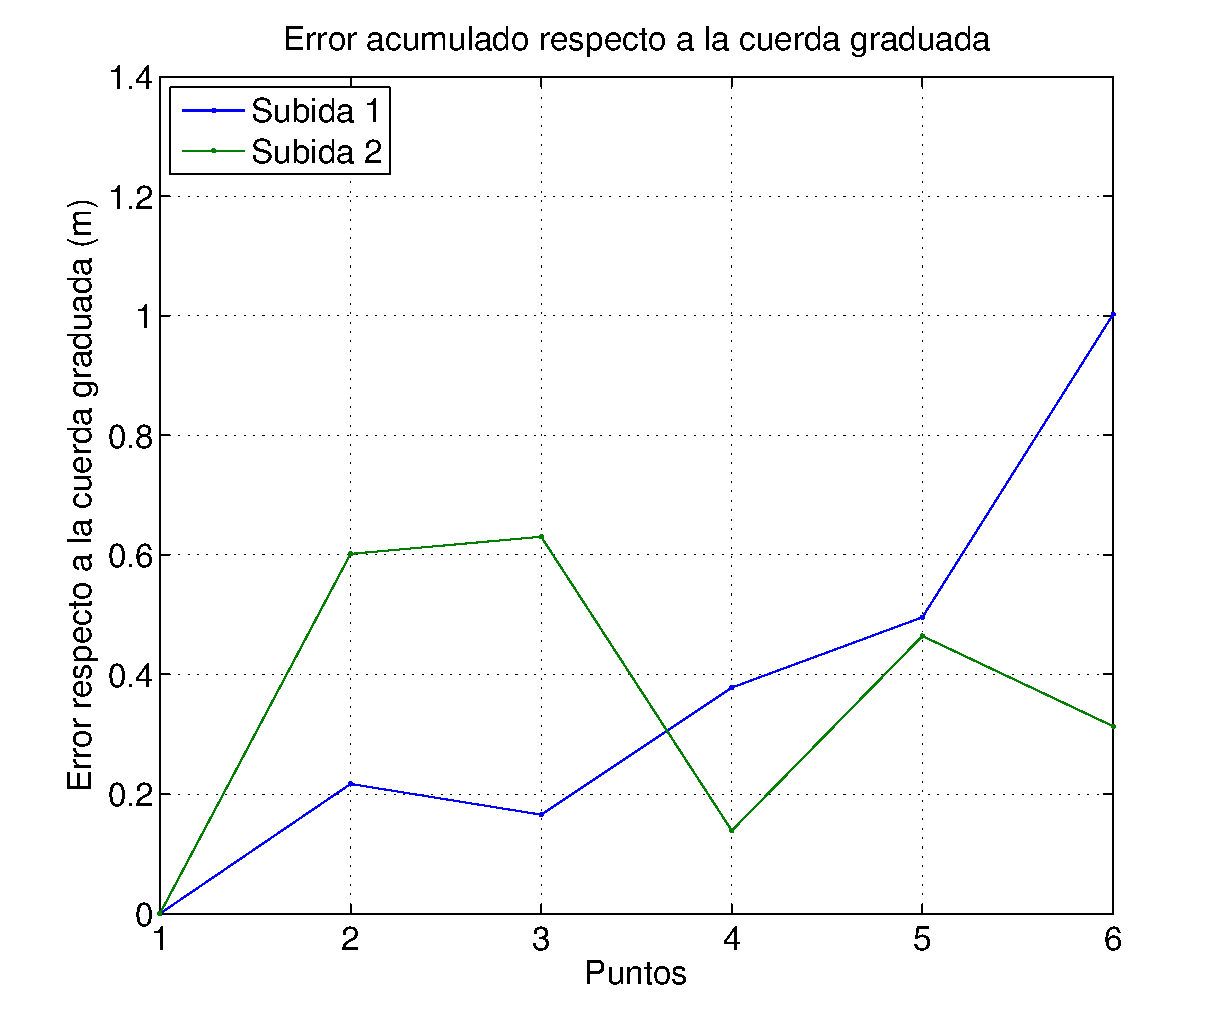
\includegraphics[width=.35\textwidth]
        {./pics_barom/1-metro-error-accum.pdf}}

	\subfloat[Error en la distancia entre pisos.]
        {\label{fig:1-metro-err-piso-a-piso.pdf}
	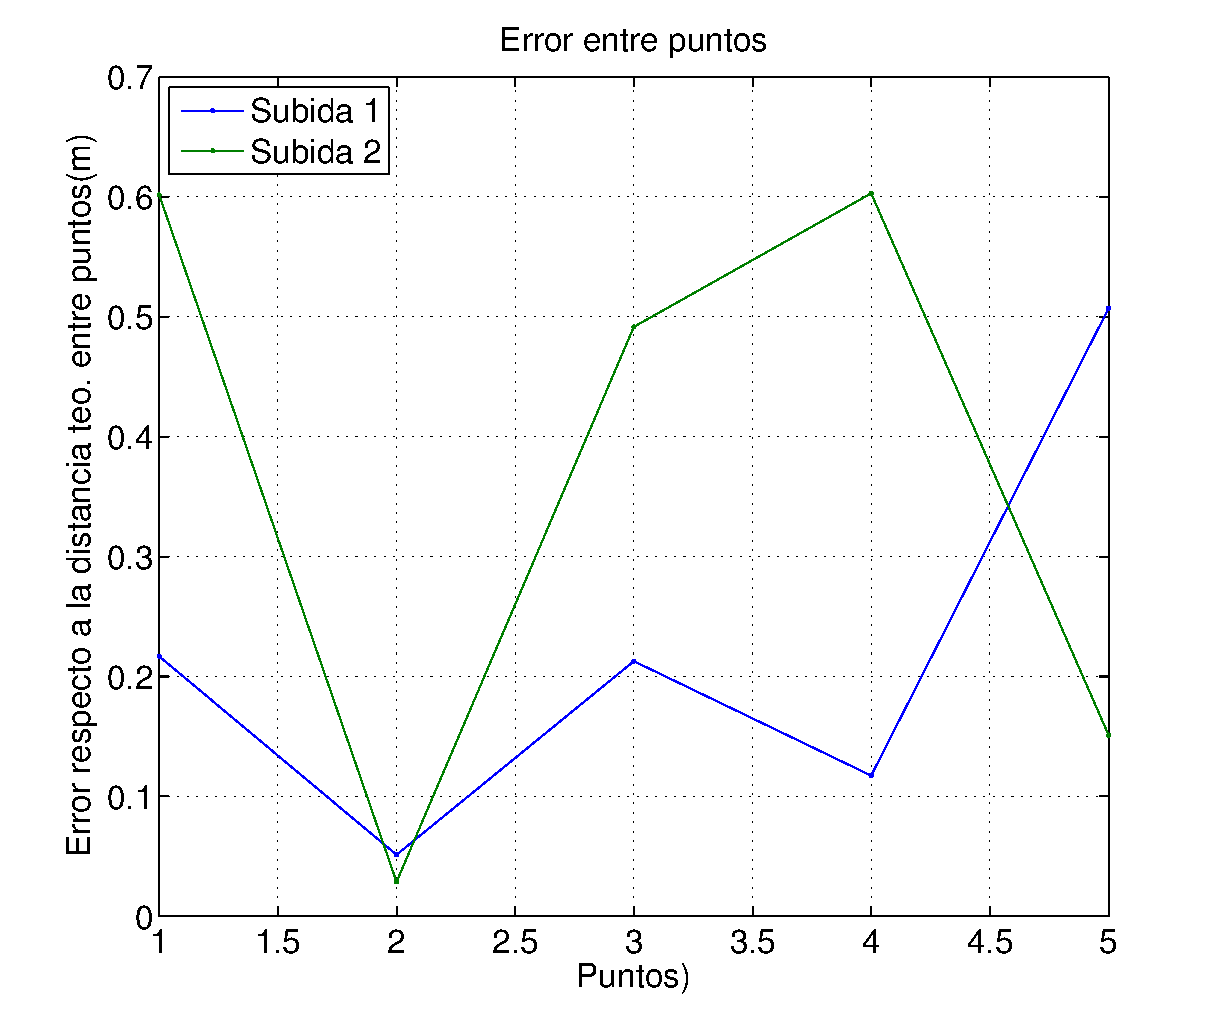
\includegraphics[width=0.35\textwidth]
        {./pics_barom/1-metro-err-punto-a-punto.pdf}}
  \caption{}
\label{fig:1-metro-err}
\vspace{-110pt}
\end{wrapfigure}

Del análisis de cada serie de manera independiente:
\begin{itemize}
\item Serie 1:
		\begin{itemize}
		\item Error promedio: $0.20m$
		\item Desviación estándar: $0.20m$
		\end{itemize}
\item Serie 2:
		\begin{itemize}
		\item Error promedio: $-0.07m$
		\item Desviación estándar: $0.49m$
		\end{itemize}
\end{itemize}

Al tener pocas muestras en cada una de las series es imposible considerarlas para armar estadísticas, de hecho ambas difieren mucho en cuanto al error promedio que presentan y la desviación estándar. 

Si se trabaja con las dos series de datos, se obtienen:

\begin{itemize}
\item Error promedio: $0.07m$
\item Desviación estándar: $0.38m$
\end{itemize}

A partir de los datos anteriores se puede concluir que el $95.5 \%$ de las veces se tiene errores inferiores a $0.76m$ en diferencias de un metro. El error se mantiene por debajo de $1m$ al usar pocas (4 muestras, 8, 10, etc) muestras para cada punto. Este error depende del drift del barómetro, y se puede reducir incorporando, de manera periódica, información externa (GPS) sobre la altura absoluta.

En la figura \ref{fig:variando} se observa la variación en la altura absoluta. Si bien cada tramo comienza y termina a una altura que cae dentro del error esperado, hay tramos del principio y del final del experimento (barómetro apoyado en el suelo) entre los que se observa una diferencia en altura de 1.5m. Esto no cae dentro del error esperado. El problema se ve luego de transcurridos varios minutos, tiempo mucho mayor al sugerido en la sección \ref{sec:caract-ruido}, puede ser causado por el drift y/o por cambios en las condiciones atmosféricas.

\begin{figure}[H]
  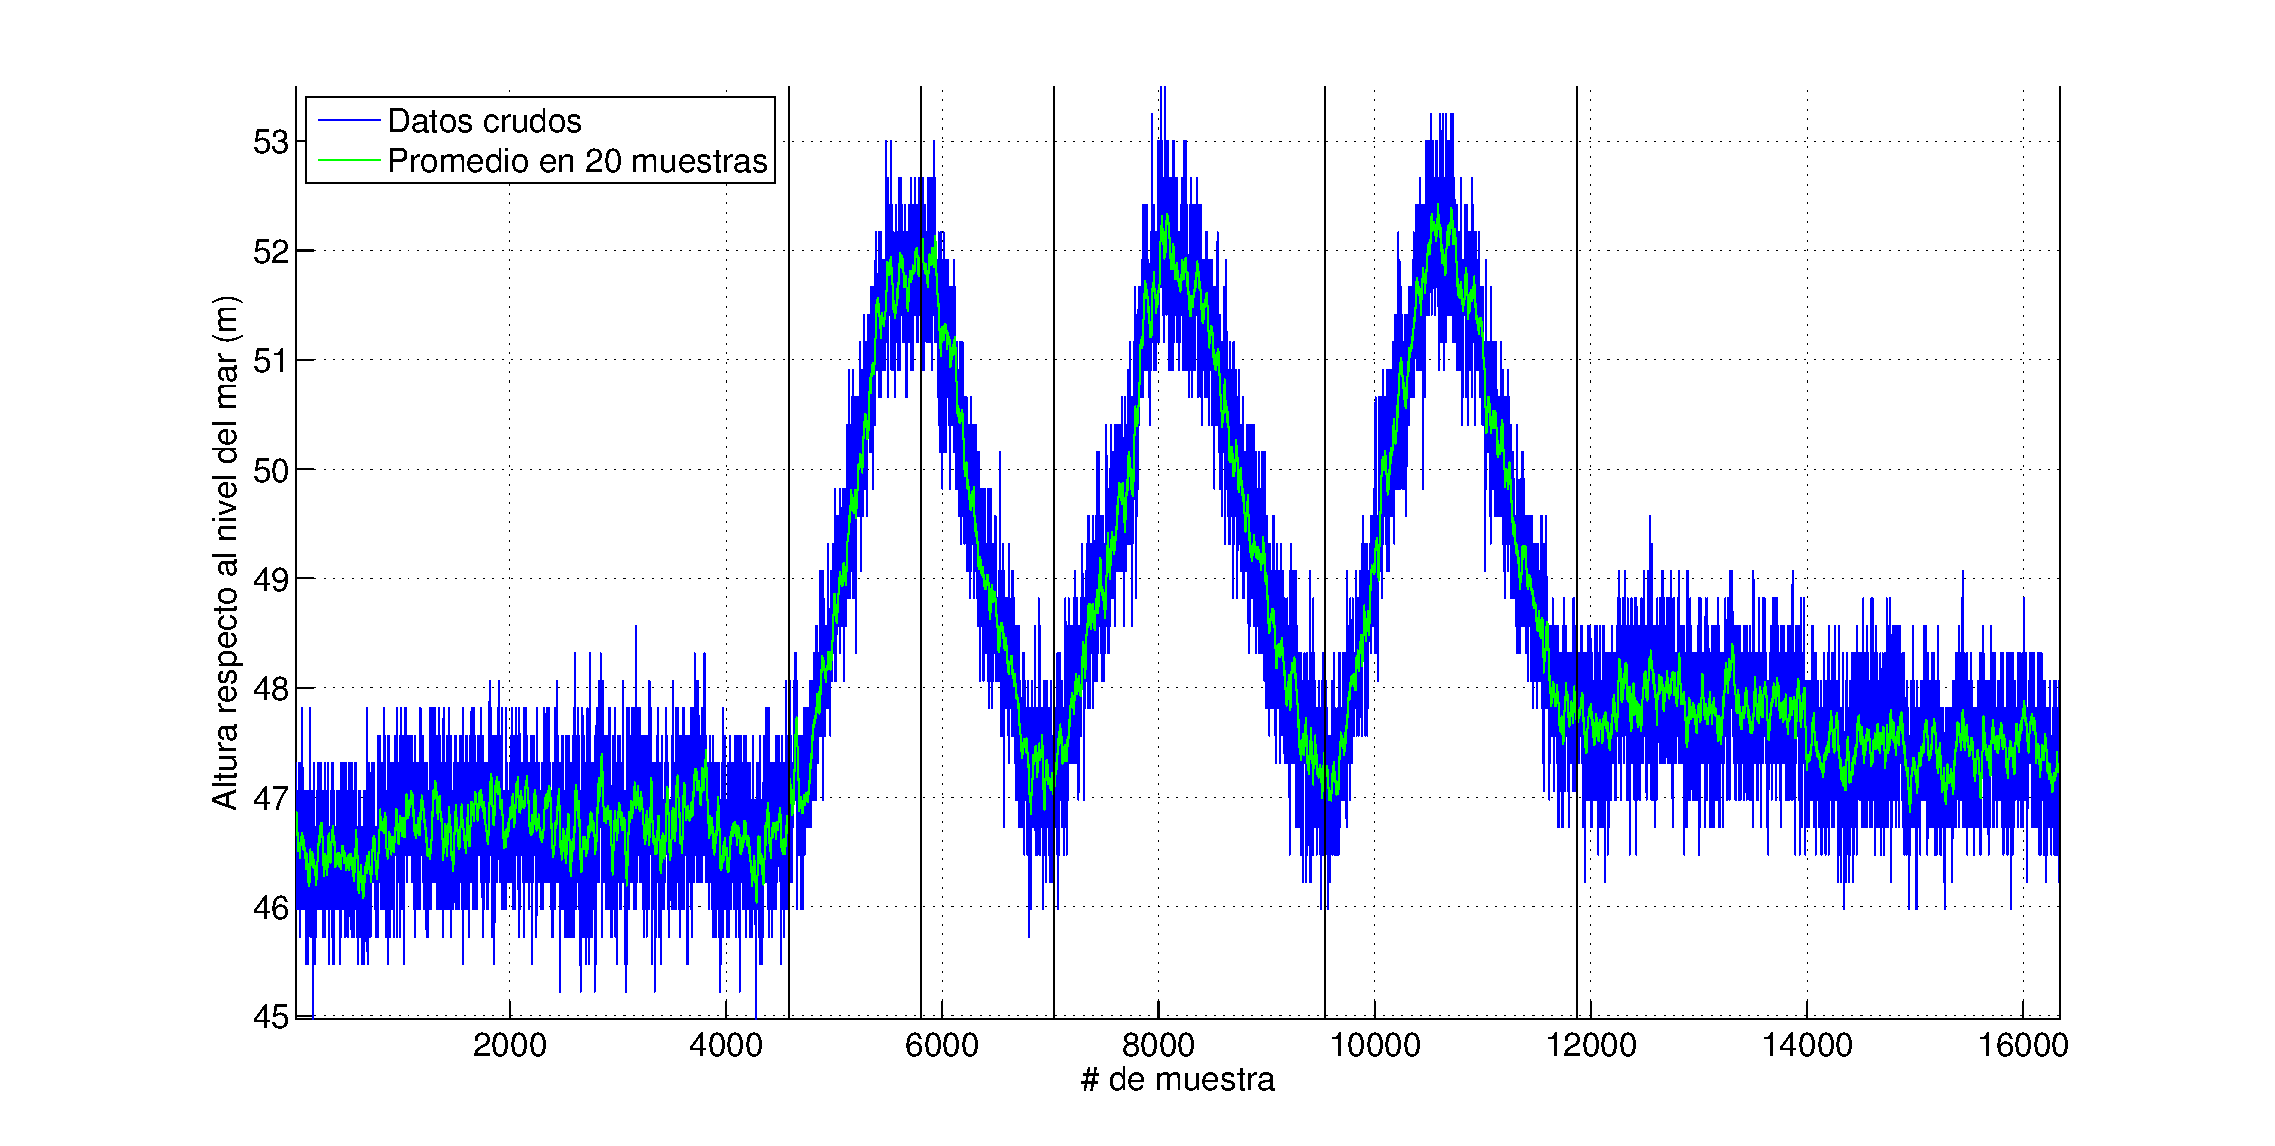
\includegraphics[width=1\textwidth]{./pics_barom/variando.pdf}
  \caption{Medidas de altura subiendo y bajando.}
  \label{fig:variando}
\end{figure}

\subsection{Distancias de decenas de centímetros}

\subsubsection{5 segundos por estante}

Se toman datos durante 5 segundos en casa escalón. Repitiendo el análisis realizado en secciones anteriores, se obtiene:
\begin{itemize}
\item Error promedio: 2.0 cm
\item Desviación estándar: 24.4 cm
\end{itemize}

\subsubsection{8 minutos por estante}

\begin{wrapfigure}{r}{0.6\textwidth}
\vspace{-90pt}
\centering
\subfloat[8 minutos por estante durante una tormenta.]{\label{fig:cm-8min-por-estante.pdf}
  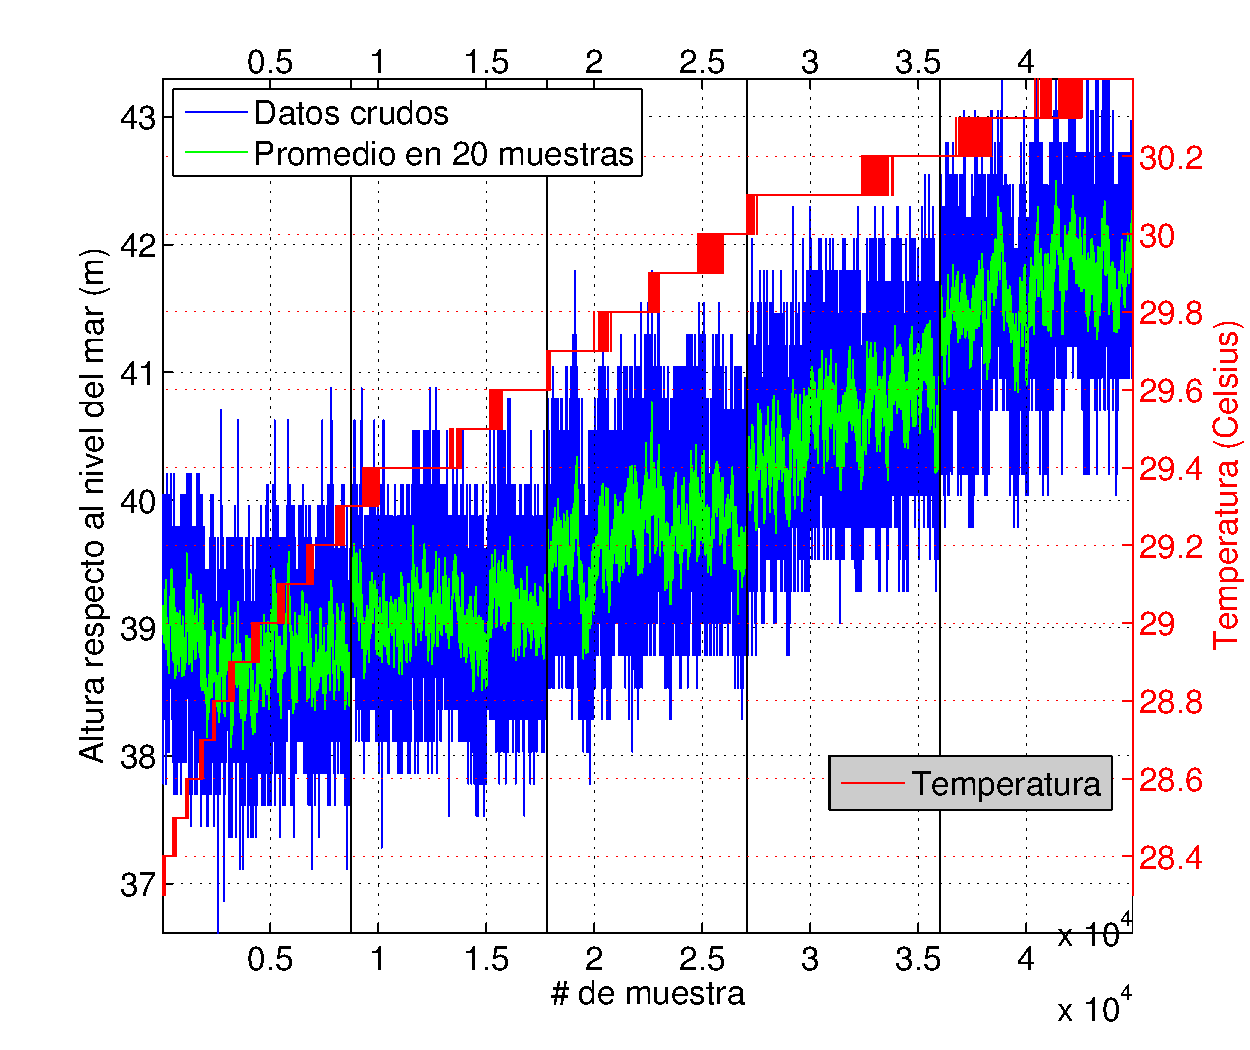
\includegraphics[width=.7\textwidth,height=.5\textwidth]{./pics_barom/cm-8min-por-estante.pdf}}
\vspace{-10pt}
\caption{}
\vspace{-10pt}
\end{wrapfigure}

En la figura \ref{fig:cm-8min-por-estante.pdf} se observan los datos capturados durante este experimento. El experimento se realiza un día de tormenta. Se toman 8 minutos de datos en cada estante, el experimento en su totalidad dura 40 minutos. El cambio de presión durante una tormenta es significativo. Se considera que esta fue la causa del drift observado en la figura \ref{fig:cm-8min-por-estante.pdf}. No se analiza el error en las medidas, ya que claramente está lejos de ser algo utilizable. Cabe destacar que no sirve tomar medidas durante tanto mucho tiempo con el barómetro, ya que el drift y/o factores externos introducen errores importantes.

\subsubsection{3m en aproximadamente 7 segundos}

\begin{wraptable}{r}{0.4\textwidth}
\vspace{-35pt}
\begin{tabular}{c|p{50pt}|p{50pt}|} 
\cline{2-3}
  & Error promedio (cm) & Desviación estándar (cm)\\ \hline
\multicolumn{1}{|c|}{$\searrow$} & 15.1 & 25.9 \\ \hline
\multicolumn{1}{|c|}{$\nearrow$} & 4.4 &  58.9 \\ \hline
\multicolumn{1}{|c|}{$\searrow$+$\nearrow$} & 10.7 & 49.0 \\ \hline
\end{tabular}
\caption{3 metros en aproximadamente 7 segundos.}
\label{tab:ruido-rms}
\vspace{-15pt}
\end{wraptable}
Como prueba extra, se recorre 4 veces la estantería sin detenerse cada estante, completando el trayecto de bajar y volver a subir en aproximadamente 7 segundos. Se calcula la distancia recorrida al bajar, la distancia recorrida al subir, y la total, y se compara dichas distancias contra los valores medidos con la cinta métrica. Los resultados se muestran en la tabla \ref{tab:ruido-rms}. Solamente se hicieron 4 experimentos, por lo que los datos estadísticos son solamente para dar una idea de la performance frente a movimientos bruscos.

Cabe destacar que el error se mantiene por debajo de los 1.2m en el peor caso.

La figura \ref{fig:estante_veloz.pdf} muestra gráficamente los resultados del experimento.

\begin{figure}[H]
\centering
  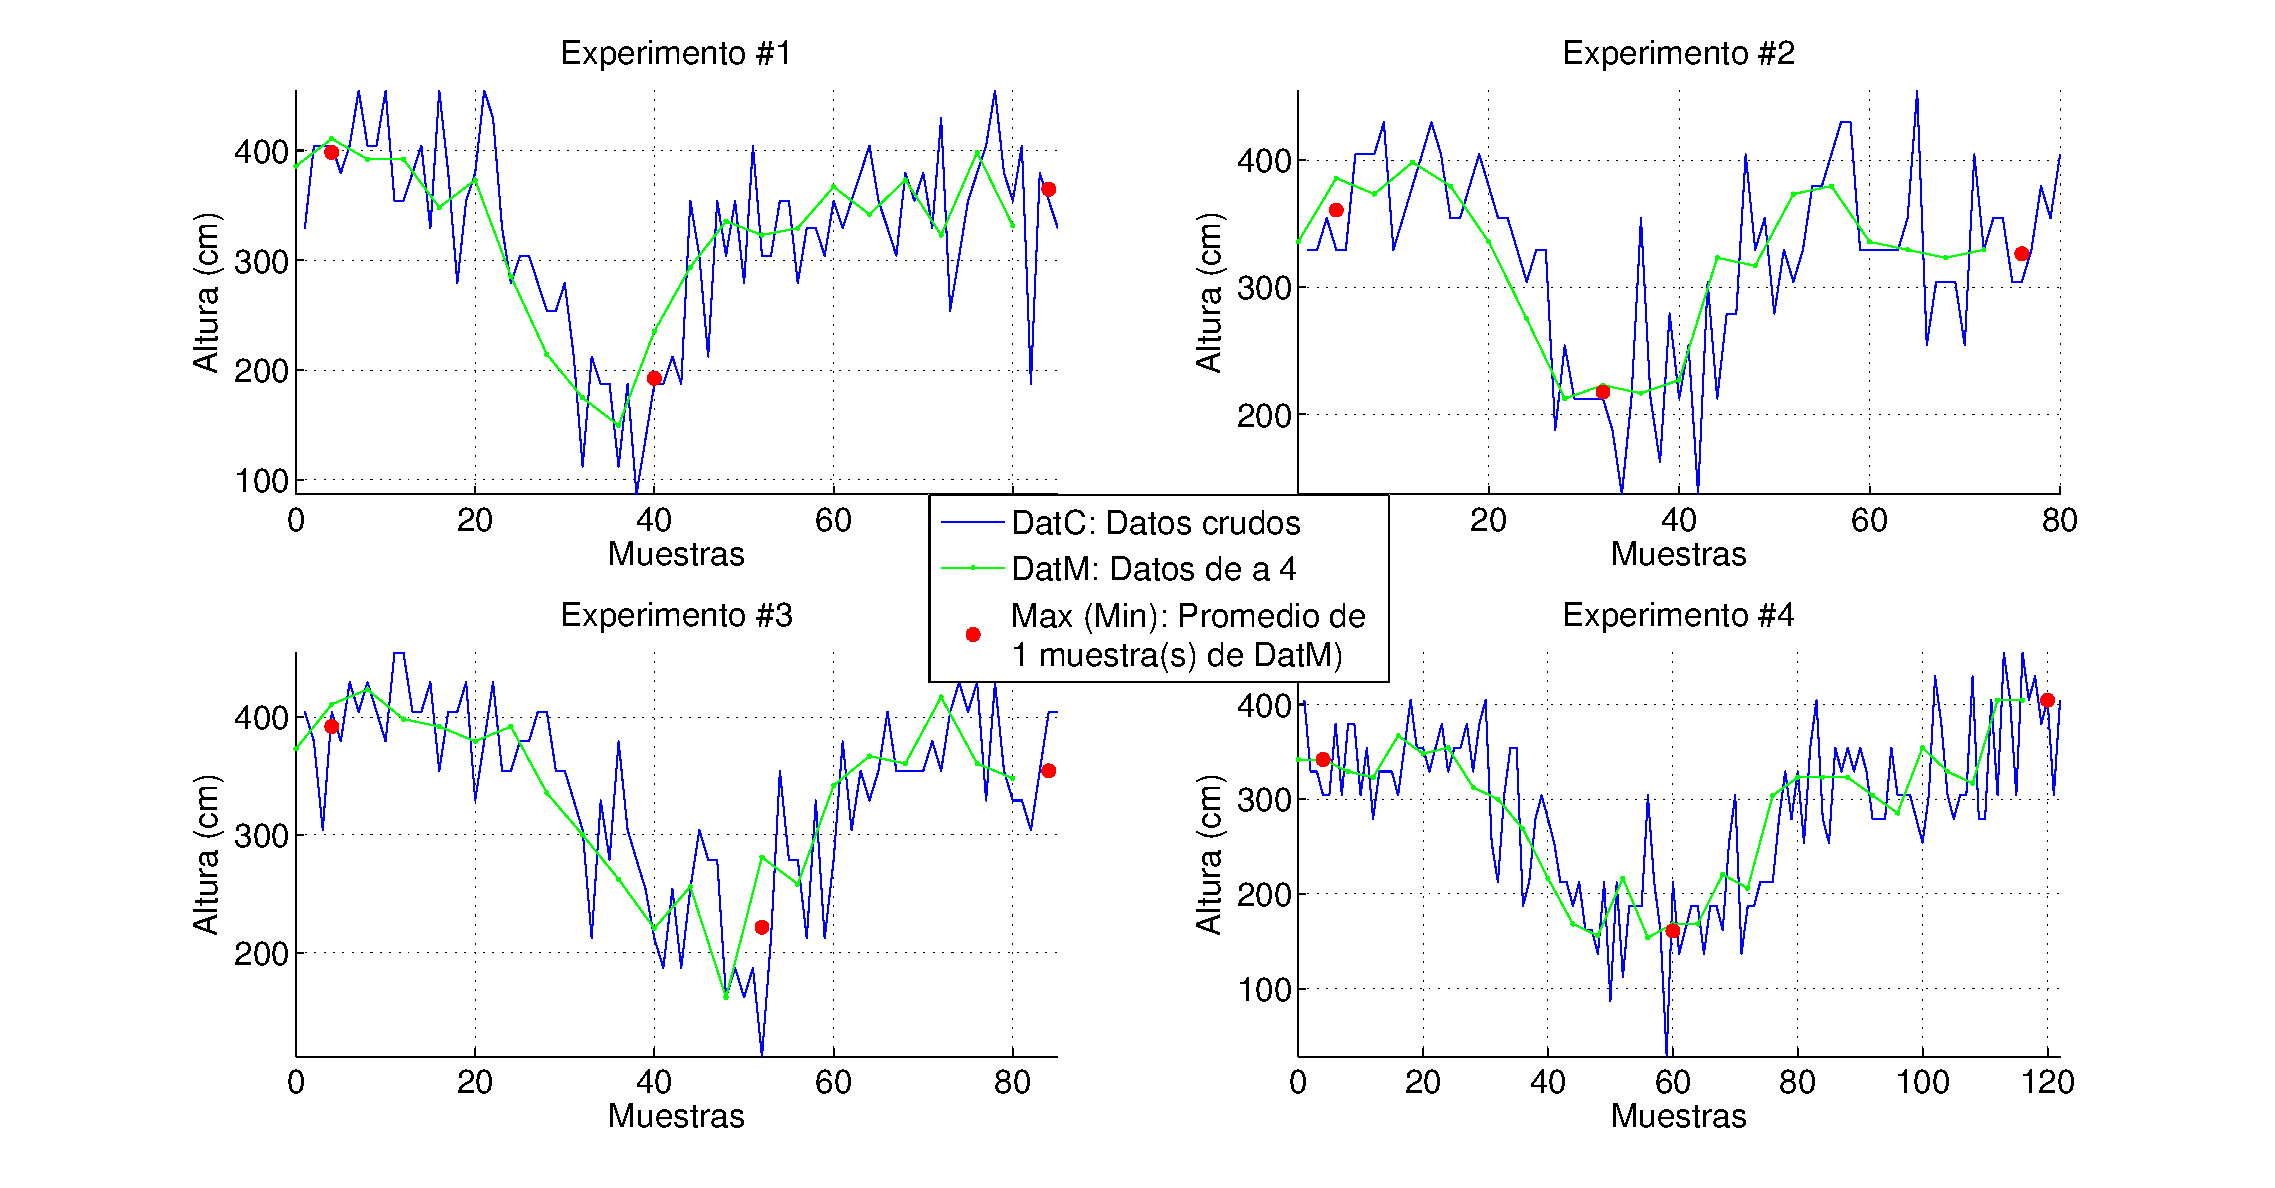
\includegraphics[width=1.1\textwidth]{./pics_barom/estante_veloz.pdf}
  \caption{3m metros en aproximadamente 7 segundos.}
  \label{fig:estante_veloz.pdf}
\end{figure}

\section{Conclusiones}
\label{sec:conclusiones}

Conclusiones más importante de las pruebas hechas con el barómetro:

\begin{itemize}
\item \textbf{Tiempo de \textit{warm-up}}: El circuito tiene un tiempo de \textit{warm-up} de aproximadamente 45 minutos, durante el cual la temperatura sube aproximadamente 1.5\degc. De las especificaciones de los sensores se deduce que una variación de temperatura tan pequeña no debería afectar la performance. De cualquier forma, es de interés analizar analizar, experimentalmente, el efecto de la variación de la temperatura sobre las lecturas de la IMU.
\item \textbf{Drift y Altura absoluta}: El drift y la sensibilidad a factores externos (clima, etc) hacen que el barómetro \textbf{no} sea adecuado para determinar la altura absoluta. No es posible obtener una mejor estimación de la altura tomando promedios durante períodos de tiempo mayores, ya que el drift introduciría errores en dicho estimador. Se observa un drift de hasta 0.5m en 1 minuto.
\item \textbf{Altura relativa}: Estando en reposo, en períodos de tiempo menores a 1 minuto es posible conocer variaciones de altura con una error menor a 0.5m.
\item \textbf{Rol del barómetro}: Se concluye que el barómetro sirve para determinar variaciones de altura, suavizando la trayectoria, mientras se espera una altura absoluta proveniente del GPS. El barómetro y el GPS se complementan. El barómetro ha de utilizarse con los siguientes parámetros:
  \begin{itemize}
  \item Error promedio: 0.5m
  \item Desviación estándar: 0.25m
  \item Modo: 0, promediando 4 muestras en la IMU.
  \item Se observa un drift de hasta 0.5m por minuto. Se debe utilizar el GPS para corregirlo.
  \end{itemize}
\end{itemize}




\end{document}